
\chapter{Problemas métricos}
	





\begin{myblock}

	\begin{figure}[H]
		\centering
		\includegraphics[width=1\textwidth]{imagenes/imagenes11/euclides-descartes.png}
	\end{figure}

\end{myblock}


\begin{myexampleblock}{Otras Geometrías}
	
\small{Euclides} (325 aC – 265 aC), en Los Elementos, partió de cinco postulados para construir la Geometría. Si alguno de esos postulados no se cumple, entonces tenemos lo que se denominan Geometrías No Euclídeas.
 
\vspace{2mm} El quinto postulado dice: \textit{“Dada una recta y un punto exterior a ella, hay una única recta que es paralela a la recta dada y que pasa por el punto”}. 

\vspace{2mm}Cuando a principios del siglo XIX se intentó demostrar el postulado por reducción al absurdo se encontró, con sorpresa, que no se llegaba a una contradicción, que se podían construir geometrías que podían no verificarlo. 

\vspace{2mm}De modo independiente, distintos matemáticos (Gauss, Lobachevsky, Bolyai...), en ese intento de demostrar el quinto postulado llegaron a la Geometría Hiperbólica. 

\vspace{2mm}La Geometría Hiperbólica es tan consistente como la Geometría Euclídea, y “su” quinto postulado es: “Dada una recta y un punto exterior a ella, existen al menos dos rectas paralelas a la dada que contienen al punto”. En la geometría hiperbólica la suma de los tres ángulos de un triángulo es menor que $180^o$. Puedes pensar en una geometría hiperbólica si te sitúas sobre una trompeta. 

\vspace{2mm}Si reescribimos el quinto postulado como: “Dada una recta y un punto exterior a ella, no existe ninguna recta paralela a la dada que contenga al punto”, se obtiene la Geometría Elíptica. 

\vspace{2mm}Imagina que estás en una esfera. Tendrás que redefinir qué entiendes como “rectas”. Si una recta es el camino más corto posible que une dos puntos, tendrás lo que se conoce como líneas geodésicas (los meridianos de un globo terráqueo). Entonces, por una de esas nuevas rectas y un punto exterior, todas las rectas que traces cortan a la primera. 

\vspace{2mm}Si lo piensas, cada vez que miras un globo terráqueo estás viendo algo de Geometría Elíptica. 

\begin{figure}[H]
		\centering
		\includegraphics[width=1\textwidth]{imagenes/imagenes11/T11IM01.png}
	\end{figure}

\vspace{2mm} Actualmente las Geometrías No Euclídeas proporcionan otras formas de entender el mundo, siendo utilizadas, por ejemplo, en Teoría de la Relatividad, o en el estudio de fenómenos ópticos y propagación de ondas. 

\vspace{2mm} \rightline{\textit{Texto: Marea Verde}\normalsize{.}}
\vspace{1mm} 
\end{myexampleblock}

\justify



Conocidos, por los dos temas anteriores, los conceptos de: 

\begin{itemize}
	
\item Vectores y sus componentes. Operaciones con vectores, geométrica y analíticamente. 
\item Productos escalar, vectorial y mixto, y su interpretación geométrica. 
\item Obtener los elementos característicos de una recta: un vector director y un punto. 
\item Obtener los elementos característicos de un plano: vector asociado, característico o normal y un punto, o dos vectores directores y un punto. 
\item Las distintas formas de expresar la ecuación de una recta y de un plano. 
\item Las posiciones relativas de rectas, de planos, y de recta y plano.
\end{itemize}


En este tema estudiaremos cómo \textbf{medir en el espacio}. La herramientas fundamentales son el \textbf{producto escalar} (la métrica: metro y goniómetro), el producto vectorial (nos proporcionará la idea de perpendicularidad) y el producto mixto de vectores (para el cálculo de volúmenes de paralelepípedos, prismas y tetraedros).

\begin{figure}[H]
		\centering
		\includegraphics[width=1\textwidth]{imagenes/imagenes11/T11IM02.png}
\end{figure}

Con esto, seremos capaces de:

\begin{itemize}
\item Hallar la distancia desde un punto a: otro punto, un plano o una recta.
\item Hallar la distancia entre rectas y planos.
\item Hallar el ángulo que forman dos rectas, dos planos o una recta con un plano.
\item Conocer las condiciones para que dos rectas sean paralelas o perpendiculares.
\item Conocer las condiciones para que dos planos sean paralelos o perpendiculares.
\item Conocer las condiciones para que una recta y un plano sean paralelos o perpendiculares.
\item Hallar la ecuación de la recta perpendicular a dos rectas (perpendicular común).
\item Hallar el punto simétrico respecto a: otro punto, una recta o un plano.
\item Calcular áreas y volúmenes.
\end{itemize}

En lo que sigue del tema, usaremos los siguientes puntos, rectas y planos (salvo que se advierta lo contrario): $P(x_0,y_0,z_0)$, $\;Q(x_1,y_1,z_1)$, $\;r:\; \{P_r,\vec v_r\}$,  $\;s:\; \{P_s,\vec v_s\}$,  $\;\pi:\; \{P_{\pi},\vec n_{\pi}\}$,  $\;\sigma:\; \{P_{\sigma},\vec n_{\sigma}\}$.

\section{Ángulos}

\begin{myblock}{Ángulos}
	\begin{figure}[H]
		\centering
		\includegraphics[width=1\textwidth]{imagenes/imagenes11/T11IM03.png}
	\end{figure}	
\end{myblock}




\subsection{Ángulo entre dos rectas}

Definimos el ángulo que forman dos rectas como aquel que forman sus vectores directores. Para asegurarnos que cogemos el menor de los dos ángulos posibles usaremos el concepto de `valor absoluto'. (Ver `producto escalar' en apartado \ref{prodesc}.)

Producto escalar: $\vec v_r \cdot \vec v_s=|\vec v_r|\;|\vec v_s|\; \cos \theta,\quad \theta=\measuredangle(\vec v_r,\vec v_s)$

\vspace{2mm}\centerline{
\colorbox{LightYellow}{
$\boxed{ \boldsymbol{ \;\theta=\measuredangle(r,s)\equiv \measuredangle(\vec v_r,\vec v_s) \; \to \; \cos \theta = \dfrac {|\;\vec v_r \cdot \vec v_s\;|}{|\vec v_r|\;|\vec v_s|}\; } }$
}}

\justify

\begin{multicols}{2}
Justificamos la formula con una imagen el caso de rectas que se cortan o se cruzan, evidentemente, para rectas paralelas o coincidentes, $\theta=0^o$, la fórmula también funciona.

	\begin{figure}[H]
		\centering
		\includegraphics[width=0.5\textwidth]{imagenes/imagenes11/T11IM04.png}
	\end{figure}	
\end{multicols}


\subsection{Ángulo entre dos planos}

Definimos el ángulo que forman dos planos como aquel que forman sus vectores asociados. Como en el caso anterior (ángulo de dos rectas),  usaremos el `valor absoluto'. 



\vspace{3mm}\centerline{
\colorbox{LightYellow}{
$\boxed{ \boldsymbol{ \;\theta=\measuredangle(\pi,\sigma)\equiv \measuredangle(\vec n_{\pi},\vec n_{\sigma}) \; \to \; \cos \theta = \dfrac {|\;\vec n_{\pi} \cdot \vec n_{\sigma}\;|}{|\vec n_{\pi}|\;|\vec n_{\sigma}|}\; } }$
}}

\justify

\begin{multicols}{2}
Como en el caso anterior, $\theta=0^o$ para planos coincidentes o paralelos, como prevé la fórmula. Para los demás (planos secantes en una recta) mostramos esta imagen.
	\begin{figure}[H]
		\centering
		\includegraphics[width=0.3\textwidth]{imagenes/imagenes11/T11IM05.png}
	\end{figure}	
\end{multicols}
	
\subsection{Ángulo entre recta y plano}


Definimos el ángulo que forman recta y plano como el `complementario' al  que forman el vector director de la recta con el vector asociado al plano.  



\vspace{3mm}\centerline{
\colorbox{LightYellow}{
$\boxed{ \boldsymbol{ \;\varphi=\measuredangle(r,\pi)\equiv 90^o-\theta,\;\theta=\measuredangle(\vec v_r,\vec n_{\pi}) \; \to \; \cos \theta = \dfrac {|\;\vec v_r \cdot \vec n_{\pi}\;|}{|\vec v_r|\;|\vec n_{\pi}|}\; } }$
}}



\justify

\begin{multicols}{2}
Evidentemente, si la recta es paralela o está contenida en el plano, 

$\vec v_r \cdot \vec n_{\pi}=0  $

$\to \vec v_r \bot \vec n_{\pi}\leftrightarrow r \;||\;\pi \to $ 

$\to\theta=90^o \Rightarrow \varphi=0^o$ 


	\begin{figure}[H]
		\centering
		\includegraphics[width=0.4\textwidth]{imagenes/imagenes11/T11IM06.png}
	\end{figure}	
\end{multicols}


\begin{table}[H]
\centering
\begin{tabular}{ccc}
\multicolumn{3}{c}{\textbf{Paralelismo y perpendicularidad entre rectas y planos}}                                                                                   \\ \\
$r\;||\;s \; \leftrightarrow \; \vec v_r \;||\; \vec v_s$                   & $\quad$ & $r \bot s \; \leftrightarrow \; \vec v_r \bot  \vec v_s$                     \\ \\
$\pi\;||\;\sigma \; \leftrightarrow \; \vec n_{\pi} \;||\; \vec n_{\sigma}$ &         & $\pi \bot \sigma \; \leftrightarrow \; \vec n_{\pi} \bot \vec n_{\sigma}$    \\ \\
$\boldsymbol{r\;||\;\pi \; \leftrightarrow \; \vec v_r \bot \vec n_{\pi}}$  &         & $\boldsymbol{r \bot \pi \; \leftrightarrow \; \vec v_r \;||\; \vec n_{\pi}}$
\end{tabular}
\end{table}


\begin{ejem}
Considera las rectas $\;r:\; (1+\lambda,2,3-\lambda)\;$, $\; s:\; (\mu,1-\mu, 2\mu)\;$ y los planos $\;\pi:\; x+y+z+3=0\;$ y $\;\sigma:\; x-2x=0\;$. Encontrar el ángulo que forman las rectas $r$ y $s$, el que forman los planos $\pi$ y $\sigma$ y el que forman la recta $r$ y el plano $\pi$.
	\end{ejem}

\noindent --- ángulo $r$ y $s$:

\noindent $\vec v_r=(1,0,-1);\; |\vec v_r|=\sqrt{2}; \quad \vec v_s=(1,-1,2);\; |\vec v_s|=\sqrt{6}$ 

\noindent $|\vec v_r \cdot \vec v_s|=|-1|=1 \to \cos \theta = \dfrac {1}{\sqrt{2}\sqrt{6}} \Rightarrow \measuredangle(r,s)=\theta=73.22^o$

\noindent --- ángulo $\pi$ y $\sigma$:

\noindent $\vec n_{\pi}=(1,1,1);\; |\vec n_{\pi}|=\sqrt{3}; \quad \vec n_{\sigma}=(1,0,-2);\; |\vec n_{\sigma}|=\sqrt{5}$ 

\noindent $|\vec n_{\pi} \cdot \vec n_{\sigma}|=|-1|=1 \to \cos \theta = \dfrac {1}{\sqrt{3}\sqrt{5}} \Rightarrow \measuredangle(r,s)=\theta=75.04^o$

\noindent --- ángulo $r$ y $\pi$:

\noindent $\vec v_r=(1,0,-1);\; |\vec v_r|=\sqrt{2}; \quad \vec n_{\pi}=(1,1,1);\; |\vec n_{\pi}|=\sqrt{3}$ 

\noindent $|\vec v_r \cdot \vec n_{\pi}|=|0|=0 \to \cos \theta = 90^o \Rightarrow \measuredangle(r,s)=90^o-\theta=0^o \leftrightarrow r\;||\; \pi$




\section[Distancias, Proyecciones Ortogonales y Simétricos]{Distancias, Proyecciones Ortogonales y Simétricos\sectionmark{Distancias}}
\sectionmark{Distancias}

\subsection{Distancia entre puntos}


Dados $P,Q \in E_3$ dos puntos del espacio, se define la distancia entre ellos como el modulo del vector que los une, es decir: 

\centerline{ \colorbox{LightYellow}{$\; d(P,Q)=|\overrightarrow{PQ}|\;$}}

\justify

\noindent \textit{Propiedades}:
$\quad d(P,Q)=d(Q,P)\; ;  \qquad  d(P,Q)=0 \leftrightarrow P=Q$.	


\subsubsection{--------- Simétrico de un punto $\boldsymbol{P}$ respecto de otro $\boldsymbol{Q}$}

Dados $P$ y $Q$, el simétrico de $P$ respecto de $Q$ será un punto $P'=sim_Q\;{P}$  tal que $Q$ sea el punto medio del segmento $\overline{PP'}$:

$\dfrac{P+P'}{2}=Q \to \;\; P'=2Q-P$



\subsection{Distancia de un punto a una recta}

\subsubsection{--------- Proyección ortogonal de un punto $\boldsymbol{P}$ sobre una recta $\boldsymbol{r}$}

Dados punto $P$ y recta $r$, buscamos el plano $\pi$ que es perpendicular a $r$ y pasa por $P$

\begin{enumerate}
\item El plano $\pi$ corta a la recta $r$ en un punto $Q$ 
\item $Q$ es la proyección ortogonal de $P$ sobre $r$.
\end{enumerate}
Ver figura en apartado siguiente.

\subsubsection{--------- Simétrico de un punto $\boldsymbol{P}$ respecto de una recta $\boldsymbol{r}$}
Dados punto $P$ y recta $r$, buscamos $Q$, la proyección ortogonal de $P$ sobre $r$, como se ha descrito anteriormente. Ahora, exigimos que $Q$ sea el punto medio del segmento formado por los puntos $P$ dado y $P'$, el simétrico que estamos buscando.

\begin{multicols}{2}

$\quad$

	\begin{enumerate}
		\item $Q$ es la proyección ortogonal de $P$ sobre $r$, $\; Q=Proy_{\;r}(P)$
		\item $P'$ será tal que $\dfrac {P+P'}{2}=Q \to P'=2Q+P$	
	\end{enumerate}

	\begin{figure}[H]
		\centering
		\includegraphics[width=0.4\textwidth]{imagenes/imagenes11/T11IM07.png}
	\end{figure}
\end{multicols}


Vamos ahora a por la \textbf{distancia de un punto $P$ a una recta $r$}, veremos \underline{tres métodos}, cada uno con sus ventajas e inconvenientes.	

\noindent MÉTODO DE LA PROYECCIÓN ORTOGONAL: Dados $P$ y $r$, buscamos $Q$, la proyección ortogonal de $P$ sobre $r$. Definimos la distancia entre punto y recta como la distancia entre el punto y su proyección ortogonal sobre la recta, de esto modo obtenemos la menor de las distancias posibles entre $P$ y un punto de $r$. $\quad \boldsymbol{ d(P,r)=d(P,Q) }\; ,\quad  Q=Proy_{\;r}(P)$

\noindent MÉTODO DEL VECTOR VARIABLE: Dados $P$ y $r$, tomamos un punto $P_r$, variable (con su parámetro $\lambda$) de la recta r con el que formamos el `vector variable' $\overrightarrow{PP_r}$ que une a $P$ con un punto cualquiera de $r$. 

\begin{multicols}{2}
Exigimos ahora que   $\overrightarrow{PP_r} \;\bot \;r$ para obtener el `punto de $r$ que está frente a $P$, eso nos determinará el $\lambda$  que define el $P_{r\bot}$ que mide la distanca mínima.

$\boldsymbol{ d(P,r)=d(P,P_{r\bot}) }\; ,\quad P_{r\bot} $ es el punto de $r$ que está frente a $P$

\begin{figure}[H]
		\centering
		\includegraphics[width=0.35\textwidth]{imagenes/imagenes11/T11IM09.png}
	\end{figure}
\end{multicols}


MÉTODO VECTORIAL: Dados $P$ y $r$, tomamos un punto determinado cualquiera $P_r\in r$,  y formamos el paralelepípedo de lados $\vec v_r$ y $\overrightarrow{PPr}$

\begin{multicols}{2}
Como el área $A$ de un paralelogramo es igual a su base $b$ por la altura $h$, calculamos el área por medio del producto vectorial, $A=|\vec v_r \times \overrightarrow{PP_r}|$, la base es $|\vec v_r|$ y la altura $h$ es la distancia buscada.

\colorbox{LightYellow}{$\boxed{\boldsymbol{d(P,r)}}=$}
$h=$
\colorbox{LightYellow}{$\boxed{\;\boldsymbol{\dfrac {|\vec v_r \times \overrightarrow{PP_r}|}{|\vec v_r|}}\;}$}

\begin{figure}[H]
		\centering
		\includegraphics[width=0.35\textwidth]{imagenes/imagenes11/T11IM10.png}
	\end{figure}
\end{multicols}

De los tres métodos visto, el primero es el más largo pero tiene la ventaja de que nos proporciona la proyección ortonormal y el simétrico de $P$ respecto de $r$ (si nos lo piden).



\subsection{Distancia de un punto a un plano}

\subsubsection{--------- Proyección ortogonal de un punto $\boldsymbol{P}$ sobre un plano $\boldsymbol{\pi}$}

Dados punto $P$ y plano $\pi$, buscamos la recta $r$ que es perpendicular a $\pi$ y pasa por $P$

\begin{enumerate}
\item La recta $r$ corta al plano $\pi$ en un punto $Q$ 
\item $Q$ es la proyección ortogonal de $P$ sobre $\pi$.
\end{enumerate}
Ver figura en apartado siguiente.

\subsubsection{--------- Simétrico de un punto $\boldsymbol{P}$ respecto de un plano $\boldsymbol{\pi}$}
Dados punto $P$ y plano $\pi$, buscamos $Q$, la proyección ortogonal de $P$ sobre $\pi$, como se ha descrito anteriormente. Ahora, exigimos que $Q$ sea el punto medio del segmento formado por los puntos $P$ dado y $P'$, el simétrico que estamos buscando.
\begin{multicols}{2}

$\quad$

\begin{enumerate}
\item $Q$ es la proyección ortogonal de $P$ sobre $\pi$.
\item $P'$ será tal que $\dfrac {P+P'}{2}=Q \;\to\; P'=2Q+P$	
\end{enumerate}

$\quad$

	\begin{figure}[H]
		\centering
		\includegraphics[width=0.5\textwidth]{imagenes/imagenes11/T11IM08.png}
	\end{figure}
	
\end{multicols}

\subsubsection{--------- Simétrico $\boldsymbol{r}'$ de una recta $\boldsymbol{r}$ respecto de un plano $\boldsymbol{\pi}$}

\begin{multicols}{2}

Basta con calcular los puntos simétricos respecto del plano de dos puntos cualesquiera de la recta y con ellos trazar la recta simétrica. Si la recta corta al plano uno de esos puntos y su simétrico pueden ser el punto de incidencia; si la recta está contenida en el plano, su simétrica es ella misma.
\begin{figure}[H]
		\centering
		\includegraphics[width=0.5\textwidth]{imagenes/imagenes11/T11IM12.png}
	\end{figure}
\end{multicols}

Otra forma de calcular la recta $t'$, simétrica de la recta $r$ respecto del plano $\pi$ es considerar $r'$ como intersección de dos planos, el propio $\pi$ y otro, $\sigma$, obtenido como aquel que contiene a $r$ y es perpencicular a $\pi$, es decir, pasa por $P_r$ y sus vectores directores son el vector director de $r$ y el vector asociado a $\pi$; esquemáticamente:

\begin{multicols}{2}



$r'\equiv Proy_{\;\pi}(r)=\begin{cases} \pi \\ \sigma \end{cases}$

donde

$\sigma:
	\begin{cases}\subset r \\ \bot \pi \end{cases} \hspace{-3mm}\equiv \begin{cases} \;\;P_r\\ \vec u=\vec v_r\\ \vec v=\vec n_{\pi} \end{cases}$

\begin{figure}[H]
		\centering
		\includegraphics[width=0.4\textwidth]{imagenes/imagenes11/T11IM12b.png}
	\end{figure}
\end{multicols}







Calculemos ahora la \textbf{distancia de un punto} $P(x_0,y_0,z_0)$ \textbf{a un plano} $\pi:\; Ax+By+Cz+D=0$, que representaremos por $d(P,\pi)$:

Dados $P$ y $\pi$, calculamos $Q=Proy_{\;\pi}(P)$, la proyección ortogonal de $P$ sobre $\pi$ y definimos la distancia del punto al plano como la distancia del punto a su proyección ortogonal en el plano, es decir, $d(P,\pi)=d(P,Q)=|\overrightarrow{PQ}|$.

Este método es largo pero tiene como contrapartida el que nos proporciona la proyección ortogonal de punto sobre plano y, con un sencillo cálculo más, el simétrico de un punto respecto de un plano.

En este caso, punto y plano, podemos obtener una \textit{fórmula} que nos facilite el cálculo de la distancia:



\noindent Sea $P_{\pi}=(x_1,y_1,z_1) \in \pi$, un punto cualquiera del plano.

\noindent Del triángulo de la figura:  $\quad cos \alpha=\dfrac {d(P,\pi)}{|\overrightarrow{PP_{\pi}} |}$

\noindent Pero también tenemos: $\quad |\;\overrightarrow{PP_\pi} \cdot \vec n_{\pi}\;|=|\overrightarrow{PP_\pi}|\;|\vec n_{\pi}|\;cos \alpha$


\begin{multicols}{2}

\noindent Luego: $\; d(P,\pi)=\dfrac {|\;\overrightarrow{PP_\pi} \cdot \vec n_{\pi}\;|}{|\vec n_{\pi}|}=\dfrac {|\;(x_0-x_1,y_0-y_1,z_0-z_1)\cdot (A,B,C)\;|}{|\vec n_{\pi}|} = \dfrac {|Ax_0+By_0+Cz_0-Ax_1-Bx_1-Cz_1|}{|\vec n_{\pi}|}$

\noindent Como $P_{\pi}\in\pi \to Ax_1+By_1+Cz_1+D=0 \to -Ax_1-Bx_1-Cz_1=D$, por lo que:


\begin{figure}[H]
		\centering
		\includegraphics[width=0.5\textwidth]{imagenes/imagenes11/T11IM11.png}
	\end{figure}
\end{multicols}



\centerline{\colorbox{LightYellow}{$\boxed{\;\boldsymbol{d(P,\pi)=
\dfrac {|\;Ax_0+By_0+Cz_0+D\;|}{|\vec n_{\pi}|}}\;}$}}
\justify
Es decir, para calcular la distancia de un punto a un plano basta con sustituir las coordenadas del punto en la ecuación del plano, considerar el resultado en valor absoluto y dividirlo por el módulo del vector asociado al plano.

\begin{ejem} Considera los puntos $A(-1,6,0)$ y $B(1,2,3)$, la recta $r:\; (1+\lambda, 2+\lambda, 3+\lambda)$ y el plano $\pi\;:x-2y+3z-4=0$

\noindent Calcula: La distancia entre $A$ y $B$, la distancia de $A$ a $r$ y a $\pi$, las proyecciones ortogonales de  $A$ sobre $r$ y sobre $\pi$ y los simétricos de $A$ respecto de $B$, respecto de $r$ y respecto de $\pi$.	
\end{ejem}

Empecemos por las proyecciones ortogonales y los simétricos:

\noindent ------ $Q_r(A):\;$ proyección de $A$ sobre $r \; \to \sigma:\; \begin{cases} A(-1,6,0) \\ \bot r \to n_{\sigma}=\vec v_r=(1,1,1) \end{cases} $ 

\noindent $1\cdot (x+1) + 1\cdot (y-6) + 1\cdot z =0 \to \;\;\sigma:\; x+y+z-5=0$

\noindent $Q_r(A)=r\cap \sigma:\quad (1+\lambda)+(2+\lambda)+(3+\lambda)-5=0 \to \;\; \lambda=-1/3$

\noindent $Q_r(A)=P_r(\lambda=-1/3)=\;(\;2/3,\;5/3,\;8/3\;)$

\noindent ------ $A'_r=simet_r(A)$, simétrico de $A$ respecto de $r$.

\noindent $\dfrac {A+A'_r}{2}=Q_r(A) \to \;\;\; A'_r=2Q_r(A)-A=\;(\;7/3,\;-8/3,\,16/3\;)$

\noindent ------ $Q_{\pi}(A):\;$ proyección de $A$ sobre $\pi \; \to s:\; \begin{cases} A(-1,6,0) \\ \bot \pi \to \vec v_s=\vec n_{\pi}=(1,-2,3) \end{cases} $

\noindent $s:\; (-1+\mu,6-2\mu,3\mu) \to Q_{\pi}=\pi\cap s:(-1+\mu)-2(6-2\mu)+3(3\mu)-4=0\to$

\noindent $\mu=7/14 \Rightarrow Q_{\pi}(A)=P_s(\mu=7/14)=\;(\;3/14,\;50/14,\;51/14\;)$

\noindent ------ $A'_r=simet_{\pi}(A)$, simétrico de $A$ respecto de $\pi$.

\noindent $\dfrac {A+A'_{\pi}}{2}=Q_{\pi}(A) \to \;\;\; A'_{\pi}=2Q_{\pi}(A)-A=\;(10/7,\;,8/7\,51/7;)$

\noindent ------ $A'_B=simet_B(A)$, simétrico de $A$ respecto de $B$.

\noindent $B$ ha de ser el punto medio de $A$ y $A'_B$, por lo que $\;\;\dfrac {A+A'_B}{2}=Q \; \to$

\noindent $ A'_B=2B-A=(3,-2,6)$

\noindent Vamos ahora a por las distancias.

\noindent ------ $d(A,B)$, distancia entre los puntos $A$ y $B$:

\noindent $d(A,B)=|\overrightarrow{AB}|=|(2,-4,3)|=\sqrt{29}\; u$

\noindent ------ $d(A,r)$, distancia de $A$ a $r$ la podemos calcular por los tres métodos, ya que tenemos la proyección ortogonal de $A$ sobre $r$ calculada en apartados anteriores.

\noindent MÉODO DE LA PROYECCIÓN ORTOGONAL: 

\noindent $\overrightarrow{ AQ_r(A) } =Q_r(A)-A=(5/3,\;-13/3,\;8/3) \to$ 

\noindent $d(A,r)=d( A,Q_r(A) )= |\overrightarrow{ AQ_r(A) }|=\sqrt{258}/3\; u$

\noindent MÉTODO DEL VECTOR VARIABLE: Tomemos un punto cualquiera de $r:\;\; A_r(1+\lambda,2+\lambda,3+\lambda)$ y formamos el vector variable $\overrightarrow{AA_r}=(2+\lambda,-4+\lambda,3+\lambda)$

\noindent Exigimos ahora que $\overrightarrow{PP_r} \bot \vec v_r \to \overrightarrow{PP_r} \cdot \vec v_r=(2+\lambda,-4+\lambda,3+\lambda)\cdot (1,1,1)=3\lambda+1=0 \to \lambda=-1/3$

\noindent El punto de $r$ que está frente a $A$ es el punto $A_{r\bot}=P_r(\lambda=-1/3)=(2/3,5/3,8/3)$

\noindent $d(A,r)=d(A,A_{r\bot})=|\overrightarrow{AA_{r\bot}}|=|(5/3,\;-13/3,\; 8/3)|=\sqrt{258} /3 \; u$

\noindent 	MÉTODO VECTORIAL: Usaremos la fórmula $d(A,r)=\dfrac{|\overrightarrow{AA_r}\times \vec v_r |}{|\vec v_r|},\;$ con $A_r$ un punto cualquiera de $r$, por ejemplo, $A_r(\lambda=0)\; (1,2,3)$

\noindent $\overrightarrow{AA_r}=A_r-A=(2,-4,3) \to \overrightarrow{AA_r}\times \vec v_r = \left| \begin{matrix} \vec i&\vec j&\vec k \\ 2&-4&3 \\ -1&6&0 \end{matrix} \right|= -7\vec i +1 \vec j +6 \vec k =(-7,1,6)$

\noindent $d(A,r)=\dfrac {|\;(-7,1,6)\;|}{|\;(1,1,1)\;|}=\dfrac {\sqrt{86}}{\sqrt{3}}=\dfrac{\sqrt{258}}{3}\; u$



\noindent ------ $d(A,\pi)$, distancia del punto $A$ al plano $\pi$, comprobemos que la distancia calculada como la que hay entre $A$ y su proyección ortogonal sobre el plano, $Q_{\pi}(A)$ coincide con la que obtenemos aplicando la fórmula $d(A,\pi)=\dfrac{|\;Ax_0+By_0+Cz_0+D\;|}{|\vec n_{\pi}|}$

\noindent $\circ\;\;d(A,\pi)=d(A,Q_{\pi}(A))=|\overrightarrow{AQ_{\pi}(A)}|= |\;(17/14,\; -34/14,\; 51/14)\;-\;(-1,6,0)\;|=|(4/7,\; -8/7,\; 12/7)|=\sqrt{4046}/14\; u$

\noindent $\circ\;\; d(A,\pi)=\dfrac{|\;Ax_0+By_0+Cz_0+D\;|}{|\vec n_{\pi}|}= \dfrac {|(-1)-2(6)+3(0)-4|}{\sqrt{14}}=\dfrac {|-17|}{\sqrt{14}}=\dfrac{17\sqrt{14}}{14}=\dfrac{\sqrt{4046}}{14}\; u$


\subsection{Distancia de una recta a un plano}

Como es obvio, si la recta está \textbf{contenida} en el plano o le es \textbf{incidente} (corta al plano), la distancia entre ambos es \textbf{cero}.
\begin{multicols}{2}
\small{Si la recta es \textbf{paralela} al plano, todos los puntos de la primera están a la misma distancia del segundo, por lo que la distancia entre ambos será la de un punto cualquiera de la recta al propio plano (nunca al revés). Para su cálculo, usaremos la fórmula de la distancia de un punto a un plano}\normalsize{.}
\begin{figure}[H]
		\centering
		\includegraphics[width=0.5\textwidth]{imagenes/imagenes11/T11IM13.png}
	\end{figure}
\end{multicols}
\noindent \small{$r\;||\;\pi \;(\vec v_r \cdot \vec n_{\pi}=0)\;\to \; d(r,\pi)=d(P_r,\pi)=\dfrac {|Ax_0+By_0+Cz_0+D|}{\sqrt{A^2+B^2+C^2}};\;P_r\in r$}\normalsize{.}

\subsection{Distancia entre planos}

\begin{multicols}{2}
Obviamente, si los planos son \textbf{coincidentes} o se \textbf{cortan} en una recta, la distancia entre ellos es \textbf{cero}. Si los planos son \textbf{paralelos} todos los puntos de uno cualquiera de ellos están a la misma distancia del otro. Para calcular la distancia entre ambos usaremos la fórmula de la distancia de un punto a un plano.

\begin{figure}[H]
		\centering
		\includegraphics[width=0.45\textwidth]{imagenes/imagenes11/T11IM14.png}
	\end{figure}
\end{multicols}

\noindent $\pi\;||\;\sigma \;\to \; d(\pi,\sigma)=d(P_\pi,\sigma)=\dfrac {|Ax_0+By_0+Cz_0+D|}{\sqrt{A^2+B^2+C^2}};\;P_{\pi}\in \pi$.



\subsection{Distancia entre rectas}

Recordemos que dos rectas pueden ocupar 4 posiciones relativas distintas en el espacio: coincidentes, secantes, paralelas o cruzarse.

Dos rectas \textbf{coincidentes} o \textbf{secantes} (que se cortan en un punto) están una respecto de otra a distancia mínima \textbf{cero}.

\begin{multicols}{2}
\small{Si las rectas son \textbf{paralelas}, todos sus puntos están a la misma distancia por lo que la distancia entre ellas será de un punto cualquiera de una de las rectas a la otra (distancia de un punto a una recta) tenemos dos métodos rápidos: el del vector variable y el método vectorial}\normalsize{.}
\begin{figure}[H]
		\centering
		\includegraphics[width=0.3\textwidth]{imagenes/imagenes11/T11IM15.png}
	\end{figure}
\end{multicols}
(repetimos la fórmula vista por este último método en este caso)

$r\;||\;s\to \;\; d(r,s)\;=\;\dfrac {|\vec v_s \times \overrightarrow{P_rP_s} |}{\vec v_s}; \quad P_r\in r$

Si las rectas \textbf{se cruzan}, el cálculo es más complicado. Desarrollaremos \underline{tres métodos para el cálculo de la distancia entre rectas que se cruzan}. Pero antes vamos a ver un ejemplo de los casos vistos anteriormente:

\begin{ejem} Sean: $\;r:\; (1+\lambda,2+2\lambda, 3+3\lambda)\;$,
$\;s:\;(\mu, 1+\mu, 3\mu)\;$, 
$\;\pi:\; 3x-z-3=0\;$ y
 $\;\sigma:\; 3x-z+4=0$. 

Calcula la distancia entre $r$ y $s$, entre $\pi$ y $\sigma$ y entre $r$ y $\pi$.
	
\end{ejem}

\noindent ------ $d(r,s):\;$ Es fácil ver que $r\; ||\; s$, por lo que la distancia entre ambas será la misma que la de un punto cualquiera de una de ellas hasta la otra de las rectas:

\noindent $r\;||\;s\to \;\; d(r,s)\;=\;d(P_r,s)\;=\;\dfrac {|\vec v_s \times \overrightarrow{P_rP_s} |}{\vec v_s}; \quad (P_r\in r)$

\noindent $P_r(1,2,3);\;\; P_s(0,1,0);\;\; \overrightarrow{PsP_r}=(1,1,3);\;\;\;\vec v_s=(1,2,3)$

\noindent $\vec v_s \times \overrightarrow{P_sP_r}=(3,0,1) \to | \vec v_s \times \overrightarrow{P_sP_r}|=\sqrt{10};\;\; \;\;|\vec v_s|=\sqrt{14}$

\noindent Luego, $\;\; d(r,s)\;=\; \dfrac {\sqrt{10}}{\sqrt{14}}=\sqrt{35}/7\; u$

\noindent ------ $d(\pi,\sigma):\; $ Ocurre que $\pi\;||\;\sigma$, por lo que la distancia entre los planos coincide con la de un punto cualquiera de uno de ellos hasta el otro plano:

\noindent $\pi\;||\;\sigma \;\to \; d(\pi,\sigma)=d(P_\pi,\sigma)=\dfrac {|Ax_0+By_0+Cz_0+D|}{\sqrt{A^2+B^2+C^2}};\;P_{\pi}\in \pi$.

\noindent $P_{\pi}(1,0,0); \qquad \sigma:\; 3x-z+4=0$

\noindent $d(\pi,\sigma)=d(P_{\pi},\sigma)=\dfrac{|3\cdot 1+0\cdot 0-1\cdot 0+4|}{\sqrt{3^3+0^2+(-1)^2}}=\dfrac{|7|}{\sqrt{10}}=7\sqrt{10}/10\; u$

\noindent ------ $d(r,\pi):\;$ Como $\vec v_r \cdot \vec n_{\pi}=(1,2,3)\cdot (3,0,-1)=0 \to r\;||\pi$, por lo que la distancia entre ambos coincide con la de un punto cualquiera de $r$ al plano $\pi$:

\noindent \small{$r\;||\;\pi \;(\vec v_r \cdot \vec n_{\pi}=0)\;\to \; d(r,\pi)=d(P_r,\pi)=\dfrac {|Ax_0+By_0+Cz_0+D|}{\sqrt{A^2+B^2+C^2}};\;P_r\in r$}\normalsize{.}

\noindent $P_r(1,2,3);\qquad \pi:\; 3x-z-3=0$

\noindent $d(r,\pi)=d(P_r,\pi)=\dfrac{|3-3-3|}{\sqrt{10}}=3\sqrt{10}/10\; u$

\vspace{3mm} \large{\textbf{Distancia entre rectas que se cruzan}}

\normalsize{Veremos} tres métodos para este cálculo: el `método de la recta perpendicular común' (más largo, pero como contrapartida nos proporciona la ecuación de la recta que es perpendicular común a dos rectas que se cruzan), el `método del plano paralelo' y el `método vectorial' (con fórmula).

\vspace{4mm} \noindent MÉTODO DE LA PERPENDICULAR COMÚN: 

$r$ y $s$ se cruzan. Vamos a buscar los puntos $R\in r$ y $S\in s$ que están \textit{`frente a frente'}, les llamaremos $R_\bot$ y $S_\bot$ y determinarán la distancia mínima entre las rectas.

\begin{myexampleblock}{Rectas que se cruzan: `perpendicular común'.}
	
	Podemos imaginar una situación física que nos aclare el método: supóngase que se quieren unir dos cables que representarán las rectas que se cruzan mediante un tercer cable que toque a ambos y que tenga la menor longitud (distancia mínima entre las rectas que se cruzan). Para ello, se conectan dos puntos cualesquiera de ambas rectas mediante un cable elástico. Si se le deja libremente tenderá a adoptar la posición de mínima energía potencial elástica (suponiendo que se puede contraer lo necesario para el caso). Esa distancia será la menor entre las rectas que se cruzan y los puntos de intersección serán los que están `frente a frente'.
	
	\begin{figure}[H]
		\centering
		\includegraphics[width=1\textwidth]{imagenes/imagenes11/T11IM16.png}
	\end{figure}
\end{myexampleblock}


\noindent Dadas $r$ y $s$ en paramétricas, tomamos un punto general (con parámetro) de cada una de ellas $R(\lambda)$ y $S(\mu)$ con los que formamos el vector \textit{`elástico'} $\overrightarrow{RS}(\lambda,\mu)$.

\noindent Para forzar a que este `vector elástico' que une dos punto cualesquiera de las rectas que se cruzan adopte la posición de mínima energía, distancia mínima entre rectas, le exigiremos que sea 	\textit{`perpendicular a ambas'}:

\vspace{2mm}\colorbox{LightYellow}{$\overrightarrow{RS} \;\bot r \ \to \overrightarrow{RS}\cdot \vec v_r=0\; \quad \wedge \quad  \overrightarrow{RS} \;\bot r
s \ \to \overrightarrow{RS}\cdot \vec v_s=0$}

\vspace{2mm}\noindent Cada una de estas imposiciones conducirá a una ecuación \textcolor{gris}{$\quad$ ($f(\lambda,\mu)=0$)} con las que formaremos un sistema de dos ecuaciones con dos incógnitas, $\lambda$ y $\mu$. \textcolor{gris}{$\quad \overrightarrow{RS}\cdot \vec v_r=0\to f_1(\lambda,\mu)=0 \; (ec.1);\quad \overrightarrow{RS}\cdot \vec v_s=0 \to f_2(\lambda,\mu)=0\; (ec.2).$}

\noindent Una vez determinados los valores de $\lambda$ y $\mu$ del sistema anterior y sustituidos en las respectivas rectas $r$ y $s$, encontramos los \textit{`puntos que están frente a frente'}, $R_\bot$ y $S_\bot$.

\noindent No queda más que definir la distancia entre las rectas que se cruzan como la que hay entre los puntos que están frente a frente: $d(r,s)=d(R_\bot,S_\bot)=|\overrightarrow{R_\bot S_\bot}|$.

\noindent Este método es un poco largo pero tiene la \textbf{ventaja} de darnos, de paso, la \textbf{ecuación de la recta perpendicular común a dos rectas que se cruzan}: si $r$ y $s$ se cruzan, la recta perpencicular común a ambas, $t$, será la recta que pasa por los puntos de $r$ y $s$ que están \textit{frente a frente}:

$\quad$ % *******************************

\begin{multicols}{2}
\noindent `perpendicular común'

\noindent $\quad t:\; \begin{cases} \; \bot \; r \\ \; \bot \; s \end{cases} \equiv t:\; \begin{cases} \; R_\bot \\ \; S_\bot \end{cases}$

 	\begin{figure}[H]
		\centering
		\includegraphics[width=.5\textwidth]{imagenes/imagenes11/T11IM18.png}
	\end{figure}
\end{multicols}

$\quad$ % *******************************

\begin{multicols}{2}
	\begin{figure}[H]
		\centering
		\includegraphics[width=.4\textwidth]{imagenes/imagenes11/T11IM20.png}
	\end{figure}
	
	$\quad$
	\begin{figure}[H]
		\centering
		\includegraphics[width=.4\textwidth]{imagenes/imagenes11/T11IM19.png}
	\end{figure}
\end{multicols}

\noindent MÉTODO DEL PLANO PARALELO:

\noindent Dadas dos rectas $r$ y $s$ que se cruzan, buscamos es plano paralelo a una de ellas que contiene a la otra. Al ser la primera recta paralela al plano buscado, todos sus puntos están a la misma distancia, por lo que la distancia entre las rectas que se cruzan coincidirá con la distancia de la primera recta al plano que contiene a la segunda y es paralelo a la primera.

\begin{multicols}{2}
\noindent $r \text{ y } s \text{ se cruzan: } \to $

\noindent $\pi:\  \begin{cases} \parallel r \\ \subset s \end{cases}  \to $

\noindent $d(r,s)=$ $d(r,\pi)=d(P_r,\pi)$ 

\noindent $(\forall P_r \in r)$

	\begin{figure}[H]
		\centering
		\includegraphics[width=.45\textwidth]{imagenes/imagenes11/T11IM22.png}
	\end{figure}
\end{multicols}

\noindent MÉTODO VECTORIAL:

\noindent $r \text{ y } s \text{ se cruzan: } \to $ Tomamos un punto de cada una de ellas y su vector director correspondiente. Con los puntos formamos un vector que une un punto de cada recta: $P_r,\;P_s,\; \vec v_r,\; \vec v_s,\; \overrightarrow{P_rP_s}$ 

\noindent El producto mixto de los tres vectores da, en valor absoluto, el volumen del paralelepípedo formado por los tres vectores, si consideramos que la base la forman los vectores  $ \vec v_r$ y $\vec v_s$, dividiendo el volumen entre el área de la base obtenemos la altura del paralelepípedo que no es más que la distancia entre las rectas que se cruzan.


\begin{multicols}{2}
$\quad$

\noindent  \colorbox{LightYellow}{$\boxed{\;d(r,s)=\;}$} $=h=\dfrac {V_{paral}}{A_{base}}=$

$\quad$
			
\noindent \colorbox{LightYellow}{$\boxed{\;=\dfrac{|\ [\vec{v_r},\ \vec{v_{s}},\ \overrightarrow{P_rP_s}]\ |}{|\ \vec{v_r} \times \vec{v_s} \ |}\;}$}

	\begin{figure}[H]
		\centering
		\includegraphics[width=.45\textwidth]{imagenes/imagenes11/T11IM21.png}
	\end{figure}
\end{multicols}


\textbf{Otro método para calcular la recta perpendicular común} a dos rectas que se cruzan es el MÉTODO DE LOS DOS PLANOS: $t$, recta perpendicular común a $r$ y $s$ que se cruzan. Evidentemente, por ser $r\bot t$ y $s \bot t$, el vector director de $t$ lo podemos obtener como producto vectorial de los vectores directores de $r$ y $s$: $\quad \vec v_t=\vec v_r \times \vec v_s$

\begin{multicols}{2}

$\quad$

\noindent \footnotesize{$t:\; \begin{cases}
 \pi     \equiv    \pi:\;  \begin{cases} \subset r \\ \subset t   \end{cases} \equiv \pi:\; \begin{cases} P_r \\ \vec v_r \\ \vec v_t=\vec v_r \times \vec v_s \end{cases}
 \\
 \sigma	 \equiv \sigma:\;  \begin{cases} \subset s \\ \subset t   \end{cases} \equiv \sigma:\; \begin{cases} P_s \\ \vec v_s \\ \vec v_t=\vec v_r \times \vec v_s \end{cases}
 \end{cases}$}

 \begin{figure}[H]
		\centering
		\includegraphics[width=.4\textwidth]{imagenes/imagenes11/T11IM17.png}
	\end{figure}
\end{multicols}


\section[Plano que equidista de dos rectas que se cruzan]
{Plano que equidista de dos rectas que se cruzan\sectionmark{Plano equidistante de dos rectas}}
\sectionmark{Plano equidistante de dos rectas}

Dadas dos rectas que se cruzan, $r$ y $s$, el plano paralelo a ambas rectas (sus dos vectores directores son los de cada uno de las rectas) que pasa por el punto medio de los puntos de $r$ y $s$ que están `frente a frente' (método de la perpendicular común) es un plano que equidista de ambas rectas. Esquemáticamente:

\noindent $\pi: \{d(\pi,r)=d(\pi,s)\} \equiv \pi:\; \begin{cases} \dfrac{R_\bot + S_\bot}{2} \\ \vec u=\vec v_r \\ \vec v=\vec v_r  \end{cases}\equiv \pi:\begin{cases} \dfrac{R_\bot + S_\bot}{2} \\ \vec n_{\pi}=\vec v_r \times \vec v_s \end{cases}$

 \begin{figure}[H]
		\centering
		\includegraphics[width=1\textwidth]{imagenes/imagenes11/T11IM23.png}
	\end{figure}


\begin{ejem}
	Calcula la distancia entre las rectas 
	
	$r:\;\dfrac{x-3}{2}=y=z-1\;\;$ y $\;\;s:\; \begin{cases} x=\mu\\y=-\mu\\z=-\mu\end{cases}$. 
	
	Calcula también la recta perpendicular común a ambas así como el plano que equidista de ellas.
\end{ejem}


\noindent $r:\; P_r(3,0,1);\;\; \vec v_r=(2,1,1);\;\; \;\;\;\;R(\lambda)=(3+2\lambda,\lambda,1+\lambda)$

\noindent $s:\; P_s(0,0,0);\;\; \vec v_s=(1,-1,-1);\;\;S(\mu)=(\mu,-\mu,-\mu)$

\vspace{5mm} \noindent MÉTODO VECTORIAL:

\vspace{3mm} \noindent $\vec v_r \times \vec v_s=\left| \begin{matrix} \vec i&\vec j&\vec k\\2&1&1\\1&-1&-1 \end{matrix} \right|=3\vec j-3\vec k=(0,3,-3)$

\noindent $|\vec v_r \times \vec v_s|=\sqrt{3^3+(-3)^2}=3\sqrt{2}$

\noindent $\overrightarrow{P_rP_s}=P_s-P_r=(-3,0,1)$

\noindent $[\vec v_r,\vec v_s,\overrightarrow{P_rP_s}]=\left|  \begin{matrix} 2&1&1\\1&-1&-1\\-3&0&-1\end{matrix} \right|=3 \to \abs{[\vec v_r,\vec v_s,\overrightarrow{P_rP_s}]}=3$

\noindent $d(r,s)=\dfrac {\abs{[\vec v_r,\vec v_s,\overrightarrow{P_rP_s}]}}{\abs{\vec v_r \times \vec v_r}}=\dfrac {\cancel{3}}{\cancel{3}\sqrt{2}}=\dfrac {\sqrt{2}}{2}\; u$

\vspace{5mm}\noindent MÉTODO DEL PLANO PARALELO:

\noindent $\pi:\;\begin{cases} \;\subset r \\ \;\parallel s \end{cases} \equiv \begin{cases} P_r((3,0,1)\\\vec v_r=(2,1,1)\\\vec v_s=(1,-1-1) \end{cases}\to$

\noindent $\left| \begin{matrix} x-3&y&z-1\\2&1&1\\1&-1&.1 \end{matrix} \right|=0 \to \cdots \to  \pi:\; y-z+1=0$

\noindent $d(r,s)=d(s,\pi)=d(P_s,\pi)=\dfrac {\abs{3\cdot 0-3\cdot 0+3}}{\sqrt{0^3+3^3+(-3)^2}}=$

\noindent $=\dfrac 3 {\sqrt{18}}=\dfrac {\cancel{3}}{\cancel{3}\sqrt{2}}=\dfrac {\sqrt{2}}{2}\; u$

\vspace{5mm}\noindent MÉTODO DE LA PERPENDICULAR COMÚN:

\vspace{3mm} \noindent $r:\; P_r(3,0,1);\;\; \vec v_r=(2,1,1);\;\; \;\;\;\;R(\lambda)=(3+2\lambda,\lambda,1+\lambda)$

\noindent $s:\; P_s(0,0,0);\;\; \vec v_s=(1,-1,-1);\;\;S(\mu)=(\mu,-\mu,-\mu)$

\noindent Formamos el vector móvil (`elástico') que une dos puntos genéricos, $R(\lambda),\; S(\mu)$, de cada recta: 

\noindent $\overrightarrow{RS}(\lambda,\mu)= S(\mu)-R(\lambda)=(-3-2\lambda+\mu,-\lambda-\mu,-1-\lambda+\mu)$

\noindent $\bullet \;\; \overrightarrow{RS}\bot \vec v_r \to \overrightarrow{RS}\cdot \vec v_r=0$

\noindent $2(-3-2\lambda+\mu)+1(-\lambda-\mu)+1(-1-\lambda+\mu)=0 \to \lambda=-7/6$

\noindent $\bullet \;\; \overrightarrow{RS}\bot \vec v_s \to \overrightarrow{RS}\cdot \vec v_s=0$

\noindent  $1(-3-2\lambda+\mu)-1(-\lambda-\mu)-1(-1-\lambda+\mu)=0 \to \mu=2/3$

\noindent Volvemos a las ecuaciones paramétricas de $r$ y $s$ con estos valores de $\lambda$ y $\mu$ para determinar los puntos de las rectas que se cruzan que está, `frente a frente':

\noindent $\lambda=-7/6 \to R_\bot(2/3,-7/6,-1/6)$

\noindent $ \mu=2/3 \to S_\bot=(2/3,-2/3,-2/3)$

\noindent $\overrightarrow{R_\bot S_\bot}=S_\bot-R_\bot=(0,1/2,-1/2) \to $

\noindent $d(r,s)=d(R_\bot,S_\bot)=\abs{\overrightarrow{T_\bot S_\bot}}=\sqrt{0^2+(1/2)^2+(-1/2)^2}=\dfrac 1 {\sqrt{2}}= \dfrac {\sqrt{2}}2\; u$

\vspace{4mm} \noindent  RECTA PERPENDICULAR COMÚN.

\vspace{3mm}\noindent $t:\;\begin{cases} \;\bot r\\ \; \bot s \end{cases} \equiv \begin{cases} R_\bot \\ S_\bot \end{cases} \equiv
 \begin{cases} R_\bot(2/3,-7/6,-1/6) \\ \vec v_t=\overrightarrow{R_\bot S_\bot}\rightsquigarrow(0,1,-1) (*) \end{cases}$
 
 \noindent (*) \textcolor{gris}{El vector $\overrightarrow{T_\bot S_\bot}$ no puede simplificarse para el cálculo de una distancia peri sí al tratarlo como vector director}.
 
\noindent $t:\; (2/3,-7/6,-1/6)+\theta (0,1,-1)$

\vspace{2mm} \noindent  MÉTODO DE LOS DOS PLANOS para el cálculo de la recta perpendicular común.

\noindent \noindent \textcolor{gris}{Este método no es adecuado para el cálculo de la distancia entre rectas que se cruzan pues no proporciona la posición de los puntos que están frente a frente}.

\noindent $t\bot r\; \wedge \; t\bot s \to \vec v_t=\vec v_r \times \vec v_t =(0,3,-3) \rightsquigarrow (0,1,-1)$

\noindent $t:\;\begin{cases} \; \bot \;r \\ \;\bot \;s \end{cases} 
\equiv 
\begin{cases}\;\pi :\begin{cases} \subset r \\  \subset t \end{cases} 
\equiv \begin{cases} P_r(3,0,1)\\ \vec v_r=(2,1,1) \vec v_t=(0.1,-1) \end{cases}
\\  
\;\sigma :\begin{cases} \subset s \\  \subset t \end{cases}
\equiv \begin{cases} P_s(0,0,0)\\ \vec v_s=(1,-1,-1) \vec v_t=(0.1,-1) \end{cases}
 \end{cases}$
 
 \noindent $\pi:\; \left| \begin{matrix} x-3&y&z-1 \\ 2&1&1 \\ 0&1&-1 \end{matrix} \right|=0 \to x-y-z-5=0$
 
 \noindent $\sigma:\; \left| \begin{matrix} x&y&z \\ 1&-1&-1 \\ 0&1&-1 \end{matrix} \right|=0 \to 2x+y+z=0$
 
 \noindent Finalmente,  $\;\;t:\; \begin{cases} \pi:\;x-y-z-5=0 \\ \sigma:\; 2x+y+z=0 \end{cases}$, que, evidentemente, coincide con la recta encontrada anteriormente en forma paramétrica (compruébese).
 

\vspace{2mm} \noindent  PLANO EQUIDISTANTE de $r$ y $s$.

\noindent 
$\tau\;$$/\;\{d(\tau,r)=d(\tau,s)\}\;$
$\begin{cases} M=\dfrac{R_\bot + S_\bot}{2}=(2/3,-11/12,-5/12) \\ \vec n_{\pi}=\overrightarrow{R_\bot S_\bot} \rightsquigarrow(0,1,-1) \end{cases}$


\vspace{3mm}\noindent $0\cdot(x-2/3)+1\cdot (y+11/2)-1\cdot(z+5/12)=0 \to \tau:\; 2x-2y+1=0$

\section{Ejercicios}

\subsection{Ejercicios resueltos}


\begin{ejre}
	Determinar la ecuación del plano que pasa por $(5,-1,0)$ y es perpendicular al vector $(7,0,4)$
\end{ejre}
\begin{proofw}\renewcommand{\qedsymbol}{$\diamond$}
	$7\cdot(x-5)+0\cdot(y+1)+4\cdot(z-0)=0 \to 7x+4z-35=0$
\end{proofw}

\begin{ejre} Determinar la ecuación de la recta $s$ sabiendo que pasa por $P$ y es perpendicular a $r$, siendo $P(2,1,0)$ y $r:(4, 4+\lambda, -1+\lambda)$	
\end{ejre}
\begin{proofw}\renewcommand{\qedsymbol}{$\diamond$}	
	$s:\; \begin{cases} P(2,1,0) \\ \bot r;\; \vec v_r=(0,1,1) \end{cases}$
	\begin{multicols}{2}
	Rectas perpendiculares a una dada hay infinitas, daremos una de ella, p.e., $\vec v_s=(3,1,-1) \quad (\vec v_r \cdot \vec v_s=0) \to $
	
	$s:\; (2,1,0)+\mu(3,1,-1)$
	 \begin{figure}[H]
		\centering
		\includegraphics[width=0.4\textwidth]{imagenes/imagenes11/T11IM24.png}
	\end{figure}
	\end{multicols}
\end{proofw}

\begin{ejre} Ecuación de la recta que pasa por $(3,0,-1)$ y es perpendicular al plano $2x-3y-z+1=0$	
\end{ejre}
\begin{proofw}\renewcommand{\qedsymbol}{$\diamond$}	

\small{$r:\; \begin{cases} P(3,0,-1) \\ \vec v_r=\vec n_{\pi}=(2,-3,-1) \end{cases}$}\normalsize{$\to$}
$(x,y,z)=(3,0,-1)+\lambda(2,-3,-1)$ 	
\end{proofw}

\begin{ejre} ¿Cuáles de las siguientes rectas se cortan, dónde y bajo qué ángulo?

a)  $(1+\lambda,  3-4\lambda, \lambda)$ y $(1+3\mu, 3, 7\mu)$  

b) $(7+\lambda, 9-2\lambda, -1)$ y $(4-3\mu, -1, 2+\mu)$
\end{ejre}
\begin{proofw}\renewcommand{\qedsymbol}{$\diamond$}	

\noindent a) $\vec v_r=(1,-4,1);\quad \vec v_s=(3,0,7);\quad \vec v_r \;\cancel{\parallel}\; \vec v_s \to $ se cortan o se cruzan.

\noindent $\overrightarrow{P_rP_s}=(1,3,0)-(1,3,0)=(0,0,0)$

\noindent Esto indica que las rectas se cortan, pues, no teniendo la misma dirección, tienen un punto en común: el punto de corte $(1,3,0)$

\noindent \textcolor{gris}{Evidentemente, $Det(\vec v_r,\vec v_s, \overrightarrow{P_rP_s})=0$, pues hay una fila de ceros en el determinante.}

\noindent Para buscar el ángulo bajo el cual se cortan usaremos el producto escalar:

\noindent $\vec v_r\cdot \vec v_s= (1,-4,1)\cdot (3,0,7)=3+0+7=10; \; \abs{\vec v_r\cdot \vec v_s}=10$

\noindent Por otro lado, $\vec v_r \cdot \vec v_s=|\vec v_r|\cdot |\vec v_s| \cos \theta = \sqrt{18}\sqrt{58}\cos \theta$

\noindent Luego $\cos \theta = \dfrac {10}{\sqrt{18}\sqrt{58}}\to \theta=72^o$

\noindent b) $\vec v_r=(1,-2,0);\quad \vec v_s=(-3,0,1);\quad \vec v_r \;\cancel{\parallel}\; \vec v_s \to $ se cortan o se cruzan.

\noindent $\overrightarrow{P_rP_s}=(4,-1,2)-(7,9,-1)=(-3,-10,3)$

\noindent $Det(\vec v_r,\vec v_s, \overrightarrow{P_rP_s})=\left| \begin{matrix} 1&-2&0\\-3&0&1\\-3&-10&3 \end{matrix}\right| =-2\neq 0 \to $ las rectas se cruzan.
\end{proofw}

\begin{ejre} Calcular el ángulo que forma la recta $(x-3)/7 = y/(-1) = (z-2)/3$ con el plano $x+3y-z+1=0$	
\end{ejre}
\begin{proofw}\renewcommand{\qedsymbol}{$\diamond$}	
$\vec v_r=(7,-1,3);\;\;|\vec v_r|=\sqrt{59}$
$\;\quad$
$\vec n_{\pi}=(1,3,-1);\;\;|\vec n_{\pi}|=\sqrt{11}$

\noindent $\vec v_r \cdot \vec n_{\pi}=7-3-3=1 \to \cos \theta=\dfrac{|1|}{\sqrt{59}\sqrt{11}} \to \;\;\theta=87.75^{\circ}$

\noindent $\varphi = \measuredangle \{r,\pi\}= 90-\theta=2'25^{\circ}$	
\end{proofw}

\begin{ejre} Dado $\pi: 2x-3y+5=0$, da las ecuaciones de:
		a) una recta paralela a él;		
		b) una recta perpendicular a él;
		c) un plano paralelo a él; 		
		d) un  plano perpendicular a él.
\end{ejre}
\begin{proofw}\renewcommand{\qedsymbol}{$\diamond$}	

Hay infinitas soluciones en todos los apartados, escribiremos una de ellas en cada caso.

\noindent a) $s:\; \begin{cases} P \to P(0,0,0) \text{ p.e.}\\ \vec v_r= (3,2,0) ; \; \vec v_r \cdot \vec n_{\pi} \end{cases} \to r:\; \dfrac{x}{3}=\dfrac{y}{2}=\dfrac{z}{0}; \quad r \parallel \pi$

\noindent b) $s:\; \begin{cases} P \to P(0,0,0) \text{ p.e.}\\ \vec v_s= \vec n_{\pi}=(2,-3,0) \end{cases} \to s:\; \dfrac{x}{2}=\dfrac{y}{-3}=\dfrac{z}{0};\quad r\bot \pi$

\noindent c) P.e., si pasa por el origen: $\quad\; \to \sigma:\; 2x-3y=0;\quad \sigma \parallel \pi$

\noindent d) $\tau:\; \begin{cases} P \to P(0,0,0) \text{ p.e.}\\ \vec n_{\tau}=(3,2,1);\; \vec n_{\tau} \bot \vec n_{\pi} \end{cases} \to \tau:\; 3x+2y+z=0;\quad \tau \bot \sigma$

	
\end{proofw}		
		

	
\begin{ejre} Calcula a para que $8$ sea la distancia entre los puntos $(a,3,-5)$ y $(7,4,1)$	
\end{ejre}

\begin{proofw}\renewcommand{\qedsymbol}{$\diamond$}	
$d(A,B)=8; \quad A(a,3,-5);\quad B(7,4,1)$

\noindent $d(A,B)=\abs{\overrightarrow{AB}}=\abs{(7-a,1,6)}= \sqrt{(7-a)^2+1^2+6^2}=\sqrt{a^2-14a+86}=8\leftrightarrow a^2-14a+86=0 \to a^2-14a+22=0 \to \begin{cases} a=7+3\sqrt{3}\\a=7-3\sqrt{3}\end{cases}$
\end{proofw}

	
\begin{ejre} Calcula el perímetro del triángulo de vértices $A(2,0,1$), $B(2,0,2)$ y $C(3,1,0)$
\end{ejre}

\begin{proofw}\renewcommand{\qedsymbol}{$\diamond$}	

$\overrightarrow{AB}=(0,0,1);\quad \overrightarrow{AC}=(1,1,-1);\quad \overrightarrow{BC}=(1,1,-2) $

\noindent $a=\abs{BC}=\sqrt{6}\; u;\quad b=\abs{AC}=\sqrt{3}\; u;\quad c=\abs{AB}=1\; u;\quad $

\noindent Perímetro $=a+b+c=\;(1+\sqrt{3}+\sqrt{6})\;\;u$

\noindent AMPLIACIÓN: `Resuelve el triángulo':

\noindent $\hat A=\angle (\overrightarrow{AB},\overrightarrow{AC}):$

\noindent $\overrightarrow{AB} \cdot \overrightarrow{AC}=\abs{ \overrightarrow{AB}} \; \abs{\overrightarrow{AC}}\; \cos A \to -1=1\cdot \sqrt{3}\cdot \cos A \to \hat A=125.3^{\circ}$

\noindent $\hat B=\angle (\overrightarrow{BA},\overrightarrow{BC}): \qquad $ \textcolor{gris}{$\overrightarrow{BA}=-\overrightarrow{AB}$}

\noindent $\overrightarrow{BA} \cdot \overrightarrow{BC}=\abs{ \overrightarrow{BA}} \; \abs{\overrightarrow{BC}}\; \cos A \to 2=1\cdot \sqrt{3}\cdot \cos B \to \hat B=35.3^{\circ}$

\noindent $\hat C=\angle (\overrightarrow{CA},\overrightarrow{CB}):\quad \hat A+\hat B+\hat C=180^o \Rightarrow \hat C=19.4^{\circ}$

\noindent El triángulo es escaleno (lados distintos) y obtusángulo (un ángulo mayor de $90^o$).

\noindent Área $=\frac 1 2 a b \sin \hat C=\frac 1 2 \sqrt{6}\sqrt{3}\sin (19.4^o)\approx 0.7\; u^2$

\noindent \textcolor{gris}{De otro modo: Área=$\frac 1 2 \; \abs{\overrightarrow{AB} \times \overrightarrow{AC}}$}; $\quad$
\noindent\textcolor{gris}{$\overrightarrow{AB} \times \overrightarrow{AC}=\left| \begin{matrix} \vec i&\vec j&\vec k \\ 0&0&1\\1&1&-1 \end{matrix} \right|=\vec j-\vec i=(-1,1,0)$}; $\quad$
\noindent \textcolor{gris}{Área $=\frac 1 2 \abs{(-1,1,0)}=\dfrac { \sqrt{2} } {2} \approx 0.7\; u^2$}

\end{proofw}

\begin{ejre} Halla la distancia de $P(5,6,6)$ a la recta $r:\  (5\lambda,\  2-\lambda,\  \lambda )$	
\end{ejre}

\begin{proofw}\renewcommand{\qedsymbol}{$\diamond$}	 
\noindent $d(P,r)=\dfrac {\abs{\overrightarrow{PP_r} \times \vec v_r }}{\abs{\vec v_r}};\quad P(5,6,6);\quad P_r(0,2,0);\quad \vec v_r=(5,-1,1)$

\noindent $\abs{\vec v_r}=\sqrt{27}=3\sqrt{3};\qquad \overrightarrow{PP_r}=P_r-P=(-5,-4,-6)$

\noindent $\overrightarrow{PP_r}\times \vec v_r=\left| \begin{matrix} \vec i&\vec j&\vec k \\ -5&-4&-6 \\ 5&-1&1 \end{matrix} \right|=-10\vec i -25 \vec j +25 \vec k =(-10,-25,25)$

\noindent $\abs{\overrightarrow{PP_r}\times \vec v_r}=\sqrt{(-10)^2+(-25)^2+25^2}=15\sqrt{6}$

\noindent $d(P,r)=\dfrac {15\sqrt{6}}{3\sqrt{3}}=5\sqrt{2}\; u$

\end{proofw}

\begin{ejre} Calcula el simétrico de $P(2,1,0)$ respecto de la recta $r:\  (5+2\lambda, \  2-\lambda, \  -2)$	
\end{ejre}

\begin{proofw}\renewcommand{\qedsymbol}{$\diamond$}	 
\noindent $P(2,1,0);\qquad P_r(5,2,-2);\quad \vec v_r=(2,-1,0)$

\noindent $\pi:\;\begin{cases}\;P\\ \bot r \end{cases}\equiv \begin{cases} \;P(2,1,0) \\ \vec v_r=(2,-1,0) \end{cases} \to $

\noindent $\to 2(x-2)-1(y-1)+0z=0 \Rightarrow \pi:\; 2x-y-3=0$

\noindent $Q=Proy_r (P)=r\cap \pi:\quad 2(5+2\lambda)-(2-\lambda)-3=0 \to $

\noindent $\to \lambda=-1 \Rightarrow Q=P_r(\lambda=-1)=(3,3,-2)$

\noindent $\dfrac {P+P'}{2}=Q \Rightarrow P'=Sim_r (P)=2Q-P=(4,5,-4)$	
\end{proofw}

\begin{ejre} Calcula las distancias entre los siguientes elementos:

	a)  $P(8,5,-6)$ y $\pi: x+2y-2z+3=0$;   		
	
	b)  $r:\  (13+12\lambda,\  2,\ 8+5\lambda)$ y $s:\  (6,\  6+\mu,\  -9)$
	
	
	c)  $r:\  (5\lambda,\  2-\lambda,\ \lambda )$ y $s:\  (5+7\mu,\  1-5\mu,\  1-5\mu)$	
	
	d)  $r:\  (1-3\lambda,\  2+\lambda, \  1-\lambda)$ y $\pi:\  x+3y=0$
	
	
	e) $r:\  (1-3\lambda,\  2+\lambda,\  1-\lambda)$ y $\pi: \ x+2y-5z-1=0$	
	
	f)  $\pi:\  y-5z+4=0$ y $\pi’:\  2y-10z=0$
	
	
	f) $\pi:\  2x-y+z=0$ y $\pi’:\  x-2y+3z=0$
\end{ejre}
	
\begin{proofw}\renewcommand{\qedsymbol}{$\diamond$}

\noindent ------ a) $d(P,r)=\dfrac {\abs{8+2\cdot 5-2\cdot (-6)+3}}{\sqrt{1^2+2^2+(-2)^2}}=11\; u$

\noindent ------ b) 
$\begin{cases}\;  r:\; P_r(13,2,8);\quad \vec v_r=(12,0,5)
\\ \; s:\; P_s(6,6,-9);\quad \vec v_s=(0,1,0) \end{cases}$

\noindent $12/0 \neq 0/1 \neq 5/0 \to \vec v_r \cancel{\parallel} \vec v_s \to $ las rectas se cortan o se cruzan.

\noindent $\overrightarrow{P_rP_s}=P_s-P_r=(-7,4,-17) \to Det(\vec v_r, \vec v_s,\overrightarrow{P_rP_s})= $

\noindent $=\left| \begin{matrix} 12&0&5\\0&1&0\\-7&4&-17 \end{matrix}\right|=-169\neq 0 \to r \text{ y } s \;$ se cruzan en el espacio.

\noindent Como solo nos piden la distancia entre las rectas, usaremos el método vectorial (fórmula):

\noindent $d(r,s)=\dfrac {\abs{[\vec v_r, \vec v_s,\overrightarrow{P_rP_s}]}}{\abs{\vec v_r \times \vec v_r}}=\dfrac {169}{13}=13\; u$

\noindent Donde hemos usado que: $\vec v_r \times \vec v_r= \left| \begin{matrix} \vec i&\vec j&\vec k\\ 12&0&5\\0&1&0 \end{matrix}\right| =-5\vec i +12 \vec j =(-5,0,12) \to \abs{\vec v_r \times \vec v_r}=\sqrt{(-5)^2+0^2+12^2}=\sqrt{169}=13$

\vspace{4mm} \noindent \textcolor{gris}{Podemos usar la fórmula del método vectorial para el cálculo de la distancia entre dos rectas en cualquier caso, no solo si las rectas se cruzan, siempre teniendo en cuanta que:}

\begin{itemize}
\item \textcolor{gris}{Si las rectas son secantes, el producto mixto sería cero: $\overrightarrow{P_rP_s}$ es combinación lineal de $\vec v_r$ y $\vec v_s$, el volumen del paralelepípedo es cero.}
\item \textcolor{gris}{En caso de rectas paralelas, al ser $\vec v_r =k\vec v_s \to $ el determinante del producto mixto sería cero (por tener dos filas iguales o proporcionales), pero también lo sería el denominador; con lo que obtendríamos la indeterminación `cero partido por cero' que nos debería hacer sospechar que las rectas son paralelas y entonces usar que $d(r,s)=d(P_r.s)$ en este caso.}
\item \textcolor{gris}{	También obtendríamos la indeterminación `cero partido por cero' si las rectas son coincidentes.}
\item \textcolor{gris}{	Conclusión: si nos piden $d(r,s)$, lo más rápido es usar la fórmula y, si aparece $\frac 0 0$ decidir si las rectas son coincidentes ($d(r,s)=0$) o si son paralelas ($d(r,s)=d(P_r,s)$). Esta última fórmula, de distancia entre rectas paralelas, también funciona para coincidentes y da cero, ya que si $r\equiv s \to P_r \in s$.}
\end{itemize}

\noindent ------ c) $\begin{cases}\; r:\; P_r(0,2,0);\quad \vec v_r=(5,-1,1) \\ \; s:\; P_s(5,1,1);\quad \vec v_s=(7,-5,-5) \end{cases} \overrightarrow{P_rP_s}=(5,-1,1)$

\noindent $\frac 5 7 \neq {-1}{-5} \neq 1 {-5} \to r \text{ y} s \;$ se cortan o se cruzan:

\noindent $Det(\vec v_r, \vec v_s,\overrightarrow{P_rP_s})= \left|\begin{matrix} 5&-1&1\\7&-5&-5\\5&-1&1 \end{matrix} \right| =0 \; $\textcolor{gris}{$[F1=F3]$}, luego las rectas $r$ y $s$ se cortan, por lo que $d(r,s)=0\; u$.

\noindent ------ d) $P_r(1,2,1); \quad \vec v_r=(-3,1,-1);\qquad \vec n_{\pi}=(1,3,0)$

\noindent $\vec v_r \cdot \vec n_{\pi}= 0 \to \vec v_r \bot \vec n_{\pi} \rightarrow \begin{cases} \; r\subset \pi \\ \; r \parallel \pi \end{cases} \to $ ¿$P_r \in \pi$?:

\noindent $1+3\cdot 2=7\neq 0 \to P_r \notin \pi \Rightarrow r \parallel \pi \Rightarrow d(r,\pi)=d(P_r,\pi)=\dfrac {\abs{1+3\cdot 2}}{\sqrt{1^2+3^2}}=\dfrac 7 {\sqrt{10}}=\dfrac {7\sqrt{10}}{10}\; u$

\noindent ------ e) $P_r(1,2,1); \quad \vec v_r=(-3,1,-1);\qquad \vec n_{\pi}=(1,2,-5)$

\noindent $\vec v_r \cdot \vec n_{\pi}=-3+2+5=4\neq 0 \to r\cap \pi$, la recta y el plano son secantes: $d(r,\pi)=0\; u$

\noindent ------ f) $\vec n_{\pi}=(0,1,-5);\qquad \vec n_{\sigma}=(0,2,-10)=-2\vec n_{\pi} \to n_{\pi} \parallel \vec n_{\sigma}$, los planos son paralelos o coincidentes.

\noindent ¿$P_{\pi} \in \sigma$:? $\pi:\; x=z=0 \to y=-4 \to P_{\pi}(0,-4,0) \to 2(-4)-10\cdot 0\neq 0 \to P_{\pi} \notin \sigma \Rightarrow \pi \parallel \sigma \longrightarrow d(\pi,\sigma)=d(P_{\pi},\sigma)= \dfrac {\abs{2(-4)-10\cdot 0}}{\sqrt{0^2+2^2+(-10)^2}}=\dfrac {8}{\sqrt{104}}=\dfrac{2\sqrt{26}}{13}\; u$ 

\noindent ------ g) $\vec n_{\pi}=(2,-1,1);\qquad \vec n_{\sigma}=(1,-2,3)$

\noindent $\frac 2 1 \neq \frac {-1}{-3} \neq \frac 1 3 \to \pi \text{ y } \sigma\;$ se cortan $\Rightarrow d(\pi,\sigma)=0\; u$
\end{proofw}

\begin{ejre}
Encuentra el valor de $k$ para que las siguientes rectas formen un ángulo de $90^{\circ}$:

$r:\; (1+2\lambda,3\lambda,4+5\lambda);\qquad s:\; (1+10\mu,2k,3-k\mu)$
\end{ejre}
\begin{proofw}\renewcommand{\qedsymbol}{$\diamond$}	
\noindent $\vec v_r=(2,3,5);\quad  \vec v_s=(10,0,k):\quad \text{ si }\measuredangle (r,s)=90^o \to  r\bot s \leftrightarrow \vec v_r\cdot \vec v_s=0 \to \vec v_r \cdot \vec v_s=20+5k=0 \Rightarrow k=-4$	
\end{proofw}

\begin{ejre}
Calcula los ángulos que forma el plano $\pi: 4x+3y+2z-1=0$ con los ejes coordenados.	
\end{ejre}
\begin{proofw}\renewcommand{\qedsymbol}{$\diamond$}
\noindent El ángulo que forman recta y plano es el complementario al que forman el vector director de la recta con el vector asociado al plano: 

\noindent $\theta=\measuredangle (\vec v_r,\vec n_{\pi}) ; \;\; \varphi = \measuredangle (r,\pi) \to \varphi=90^{\circ}-\theta$

\noindent 	$\vec n_{\pi}=(4,3,2); \quad \vec i=(1,0,0);\;\; \vec j=(0,1,0);\;\; \vec k=(0,0,1)$

\noindent $\vec n_{\pi}\cdot \vec i = |\vec n_{\pi}|\;|\vec i|\; \cos \theta_X \to 4=\sqrt{33}\cdot 1 \; \cos \theta_X \to \theta_X=45.87^o$

\noindent $\vec n_{\pi}\cdot \vec j = |\vec n_{\pi}|\;|\vec i|\; \cos \theta_X \to 3=\sqrt{33}\cdot 1 \; \cos \theta_Y \to \theta_X=58.52^o$

\noindent $\vec n_{\pi}\cdot \vec k = |\vec n_{\pi}|\;|\vec i|\; \cos \theta_X \to 2=\sqrt{33}\cdot 1 \; \cos \theta_Z \to \theta_X=69.63^o$

\noindent Luego los ángulos son:  $\varphi_X=90-45.87=44.13^o;\quad$ 
$\varphi_Y=90-55.82=34-18^o;\quad$ 
$\varphi_Z=90-69.63=20.37^o$ 
\end{proofw}

\begin{ejre} Determina el valor de $t$ para que las siguientes rectas formen un ángulo de $60^o$	

$r:\; (1+\lambda,2-\sqrt{2}\lambda,3-\lambda); \quad s:\;(1+\mu, 2+t\mu,3+\mu)$

¿Las recta se cortan en un punto o se cruzan en el espacio?
\end{ejre}
\begin{proofw}\renewcommand{\qedsymbol}{$\diamond$}	
\noindent	$\vec v_r=(1,-\sqrt{2},-1);\quad \vec v_s=(1,t,1)$

\noindent $\vec v_r \cdot \vec v_s=1-\sqrt{2}t-1=\sqrt{2}t$

\noindent $|\vec v_r|\;|\vec v_s|\;\cos \theta=2\sqrt{2+t^2}\cos 60^o=\sqrt{2+t^2}$

\noindent $\cos \theta = \dfrac {\abs{\vec v_r \cdot \vec v_s}}{|\vec v_r|\;|\vec v_s|}\to \dfrac 1 2 = \dfrac {\abs{\sqrt{2}t}}{2\cdot \sqrt{2+t^2}} \to $

\noindent $\to \begin{cases} \sqrt{2}t=\sqrt{2+m^2} &\to\;\; m=\sqrt{2} \\ \sqrt{2}t=-\sqrt{2+m^2} &\to\;\; m=-\sqrt{2} \end{cases}$

\noindent Como $(1,2,3)\in r\;\wedge \; (1,2,3)\in s \to r\cap s=P(1,2,3)$, las rectas se cortan.

\noindent \textcolor{gris}{Como, en este caso, resulta evidente que (1,2,3) es un punto de ambas rectas, tenemos dos rectas que forman $60^o$ y tienen un punto en común por lo tanto, se cortan. No es necesario comprobar que $Det(\vec v_r, \vec v_s, \overrightarrow{P_rP_s}=0$.}
\end{proofw}

\begin{ejre}
Calcula,  la distancia	entre las rectas:

$r:\; (4\lambda,-10-3\lambda,9+5\lambda);\quad s:\; (2-12\mu, 1+9\mu,4+\mu)$
\end{ejre}
\begin{proofw}\renewcommand{\qedsymbol}{$\diamond$}	
\noindent Usaremos,esta vez, el método del plano paralelo.

\noindent $\pi:\;\begin{cases} \subset r \\ \parallel s \end{cases} \to d(r,s)=d(P_s,\pi)$

\noindent  $\pi:\;\begin{cases} \subset r \\ \parallel s \end{cases} \equiv \begin{cases} P_r(0,-10,9) \\ \vec u=\vec v_r=(4,-3,5) \\ \vec v=\vec v_s=(-12,9,1) \end{cases} \to $

\noindent $\to \left| \begin{matrix} x&y+10&z-9\\4&-3&5\\-12&9&1 \end{matrix} \right|=0 \to \pi:\; 3x+4y+40=0$

\noindent $d(r,s)=d(P_r,\pi)=\dfrac {\abs{3\cdot 2+4\cdot 1+0\cdot 4+40}}{\sqrt{3^2+4^2+0^2}}=\dfrac {50}{5}=10\; u$

\noindent \textcolor{gris}{Se sugiere al lector/a que resuelva el problema por los otros dos métodos.}
\end{proofw}

\begin{ejre}
	Calcula el volumen del tetraedro que forma el plano $4x+6y+5z-60=0$ con los ejes coordenados.
\end{ejre}
\begin{proofw}\renewcommand{\qedsymbol}{$\diamond$}	
\noindent Encontremos los vértices, que junto al origen, $\mathcal O=(0,0,0)$, formarán el tetraedro.

\noindent $Z:\; x=0 \;\wedge\; y=0 \to \pi:\; z=12\to A(0,0,12)$

\noindent $X:\; y=0 \;\wedge\; z=0 \to \pi:\; x=15\to A(15,0,0)$

\noindent $Y:\;x=0 \;\wedge\; z=0 \to \pi:\; z=10\to A(0,10,0)$
\begin{multicols}{2}
\begin{figure}[H]
		\centering
		\includegraphics[width=0.5\textwidth]{imagenes/imagenes11/T11IM25.png}
	\end{figure}
 $\overrightarrow{OA}=(0,0,12)$

 $\overrightarrow{OB}=(15,0,0)$

$\overrightarrow{OC}=(0,10,0)$

$[\overrightarrow{OA},\overrightarrow{OB},\overrightarrow{OC}]= $

$=\left| \begin{matrix} 0&0&12\\15&0&0\\0&10&0 \end{matrix}\right|=-1800$
\end{multicols}
\noindent $V_{tetraedro}=\dfrac 1 6 \;\abs{[\overrightarrow{OA},\overrightarrow{OB},\overrightarrow{OC}]}=\dfrac {|-1800|}{6}=300\; u^3$
\end{proofw}

\begin{ejre}
	Encuentra la ecuación del plano $\pi$ perpendicular a la recta $r:\; \dfrac{x+3}{2}=\dfrac{y-4}{3}=\dfrac{z}{4}$ y que pasa por el punto $P(-1,1,0)$. Calcula, así mismo, el volumen del tetraedro que forma el plano $\pi$ al cortar a los ejes coordenados.
\end{ejre}
\begin{proofw}\renewcommand{\qedsymbol}{$\diamond$}	
\noindent $\pi:\; \begin{cases} \bot r \\ \;P \end{cases}\equiv \begin{cases} \vec n_{\pi}=\vec v_r=(2,3,4) \\ P(-1,1,0) \end{cases} \to$

\noindent $2(x+1)+3(y-1)+4z=0 \to \pi:\; 2x+3y+4z-1=0$

\noindent $X\cap \pi \;\;  (y=0,\; z=0 \to x=1/2) \to \; A(1/2,0,0)$

\noindent $Y\cap \pi \;\;  (x=0,\; z=0 \to y=1/3) \to \; B(0,1/3,0)$

\noindent $Z\cap \pi \;\;  (x=0,\; y=0 \to z=1/4) \to \; A(0,0,1/4)$

\noindent $V=\dfrac 1 6 \; \abs{\; \left| \begin{matrix} 1/2&0&0\\0&1/3&0\\0&0&1/4 \end{matrix} \right|\; }=\dfrac {\abs{\dfrac {1}{24}}}{6}=\dfrac {1}{144}\; u^3$
 
\end{proofw}

\begin{ejre}.
	
	a) Encuentra la ecuación del plano $\pi$ que contiene a la recta $r:\; \begin{cases}x+y-z+1=0\\x+2y+z=0 \end{cases}$ y es perpendicular al plano $\sigma:\; 2x-y+3z+1=0$.
	
	b) Obtén las ecuaciones paramétricas de la recta $s$ formada por $\pi$ y $\sigma$.
	
	c) Determina el ángulo que forma la recta $r$ con el plano $\sigma$
\end{ejre}
\begin{proofw}\renewcommand{\qedsymbol}{$\diamond$}	
	
\begin{multicols}{2}
\begin{figure}[H]
		\centering
		\includegraphics[width=0.4\textwidth]{imagenes/imagenes11/T11IM26.png}
	\end{figure}

$\pi:\;\begin{cases} \subset r \\ \bot \sigma \end{cases} \equiv$

$\equiv \begin{cases} P_{r_1}(1,-1,1) \\ \vec u=\vec v_r=(2,-1,3) \\ \vec v=\vec n_{\pi}=(2,1,3) \end{cases}$

\end{multicols}

\noindent Donde $r:\; x=1\to \begin{cases} y-z=-2\\2y+z=-1 \end{cases} \to y=-1; \; z=1 \to P_{r_1}(1,-1,1)$

\noindent  $r:\; x=4\to \begin{cases} y-z=-5\\2y+z=-4 \end{cases} \to y=-3; \; z=2 \to P_{r_2}(4,-3,2)$

\noindent $\vec v_r=\overrightarrow{P_{r_1}P_{r_2}}=(3,-2,1)\; \quad \vec n_{\pi}=(2,-1,3)$

\noindent ------ a) $\;\left| \begin{matrix} x-1&y+1&z-1\\2&-1&3\\2&1&3 \end{matrix}\right|=0 \to \pi:\; 5x+7y-z+3=0$

\noindent ------ b) $s:\; \begin{cases} \pi:\; 5x+7y-z+3=0\\ \sigma:\; 2x-y+3z+1=0 \end{cases}$

\noindent $y=0 \to \begin{cases} 5x-z=-3 \\ 2x+3z=-1 \end{cases} \to P_{s_1}( -10/17,0,1/17 )$ 

\noindent $y=1 \to \begin{cases} 5x-z=-10\\ 2x+3z=0 \end{cases} \to P_{s_1}( -30/17,1,20/17 )$ 

\noindent $\vec v_s=\overrightarrow{P_{r_1}P_{r_2}}=(-20/17, 1, 19/17) \rightsquigarrow  (-20,17,19)$

\noindent $s:\: \begin{cases} P_s(-10/17,0,1/17) \\ \vec v_s=(-20,17,19) \end{cases} \to s:\; \begin{cases} x=-10/17-20\lambda \\y=17\lambda \\ z=1/17+19\lambda \end{cases}$

\noindent ------ c) $\measuredangle(r,\sigma)=\varphi=90^o-\measuredangle(\vec v_r,\vec n_{\sigma})=90^o-\theta$

\noindent $\cos \theta=\dfrac {\abs{\vec v_r \cdot \vec n_{\pi}}}{ |\vec v_r|\;|\vec n_{\pi}|}=\dfrac {|(3,-2,1)\cdot (2,-1,3)|}{\sqrt{14} \sqrt{14}}=\dfrac 1 2 \to \theta = 60^o \Rightarrow \varphi =30^o$

\end{proofw}

\begin{ejre}
	Sea $r:\; \begin{cases} x-2z+3=0\\y-z-4=0\end{cases}\; $ y $\pi:\; x+2y+3z-1=0$. Encuentra la ecuación de la recta $s$ situada en $\pi$, que pase por $P(2,1,-1)$ y que sea perpendicular a $r$.
\end{ejre}
\begin{proofw}\renewcommand{\qedsymbol}{$\diamond$}	
\noindent $r:\; z=0\to y=4,\; x=-3:\; P_{r_1}(-3,4,0); \quad z=1 \to y=5,\; x=-1:\; P_{r_2}(-1,5,1) \Rightarrow \vec v_r=\overrightarrow{P_{r_1}P_{r_2}}=(2,1,1)$
 
\noindent $\vec v_s=\vec v_r \times \vec n_{\pi}$, así, $s\bot r$ y $s \subset \pi$.

\noindent \textcolor{gris}{También podríamos haber hallado $\vec v_r$ buscando una solución particular del SEL homogéneo asociado a $r$ o mediante el producto vectorial de los dos vectores directores de los planos que definen a $r$.}
	
\noindent $\vec v_s= \left| \begin{matrix} \vec i & \vec j & \vec k \\ 2&1&1 \\ 1&2&3 \end{matrix} \right|=(1,-5,3)$

\noindent $s:\; \begin{cases} P \\ \subset \pi \\ \bot r \end{cases} \equiv \begin{cases} \;\; P \\ \vec v_s=\vec v_r \times \vec n_{\pi} \end{cases} \to X=(2,1,-1)+\lambda(1,-5,3)$
\end{proofw}


\begin{ejre}
	Encuentra la recta perpendicular común a las rectas: 
	
	$r:\;\begin{cases}x+y-z-4=0\\x+2y-7=0\end{cases}; \quad s:\;\begin{cases} x-2=0\\y+3=0 \end{cases}$
	
	Determina, también, el plano que equidista de ambas rectas.
\end{ejre}
\begin{proofw}\renewcommand{\qedsymbol}{$\diamond$}	
\noindent Busquemos punto y vector director de cada recta para escribirlas en paramétricas.

\noindent $r:\;\begin{cases}x+y-z-4=0\\x+2y-7=0\end{cases} \to \begin{cases} P_{r_1}(1,3,0) \\ P_{r_2}(3,2,1) \end{cases} \to \vec v_r=(2,-1,1)$

\noindent $s:\;\begin{cases}x-2=0\\y+3=0\end{cases} \to \begin{cases} P_{s_1}(2,-3,0) \\ P_{s_2}(2,-3,1) \end{cases} \to \vec v_s=(0,0,1)$

\noindent $r$ y $s$ en paramétricas son:

\noindent $r:\; \begin{cases} x=1+2\lambda \\ y=3-\lambda \\ z=\lambda \end{cases}; \quad s:\; \begin{cases} x=2\\y=-3\\z=\mu \end{cases}$

\noindent Tomamos un punto genérico de cada recta para formar el vector móvil (`elástico') que los une:

\noindent $\begin{cases} R(\lambda)=(1+2\lambda,3-\lambda,\lambda) \\ S(\mu)=(2,-3,\mu) \end{cases} \to$

\noindent $ \overrightarrow{RS}(\lambda, \mu)=(1+2\lambda, -6+\lambda, \mu-\lambda) $

\noindent Exigimos ahora que $\overrightarrow{RS}$ sea perpendicular a $r$ y a $s$:

\noindent $\overrightarrow{RS}\bot r \leftrightarrow \overrightarrow{RS}\cdot \vec v_r=0 \to -6\lambda+\mu+8=0$

\noindent $\overrightarrow{RS} \bot s \leftrightarrow \overrightarrow{RS} \cdot \vec v_s=0 \to \mu-\lambda=0$

\noindent $\begin{cases} -6\lambda+\mu+8=0 \\ \mu-\lambda =0 \end{cases} \to \lambda=\mu=\dfrac 8 5$

\noindent Determinamos, con estos valores de los parámetros, los puntos de $r$ y $s$ que están `frente a frente':

\noindent $R_\bot=R(\lambda=8/5)=(21/5,\; 7/5,\; 8/5)$

\noindent $S_\bot=S(\mu=8/5)=(2,-3,\; 8/5)$

\noindent $\vec v_t=\overrightarrow{R_\bot S_\bot}=(-11/5,-22/5,0) \rightsquigarrow  (1,2,0); \quad t:\begin{cases} \bot r \\ \bot s \end{cases}$

\noindent Finalmente, la recta perpendicular común a las dos rectas dadas es: $t:\; (2,-3,\; 8/5)+\theta (1,2,0)$

\noindent \textcolor{gris}{Se sugiere que el/la lector/a encuentren la recta perpendicular común a $r$ y $s$ por el método de los dos planos.}

\noindent El plano $\pi$ que equidista de ambas rectas es el que pasa por el punto medio de los puntos que están `frente a frente', $M_{R_\bot S_\bot}=\dfrac {R_\bot + S_\bot}{2}=(31/10,\; -4/5, \;0)$ y tiene por vector asociado el vector que los une, $\vec n_{\pi}= \overrightarrow{R_\bot S_\bot}  \rightsquigarrow  (1,2,0)$

\noindent $1(x-31/10)+2(y+4/5)+0(z)=0 \to \pi:\; 10x+20y-47=0$
\end{proofw}


\begin{ejre}
	Determina el valor de $t$ para que las rectas $r:\; (2\lambda, 1-\lambda,\lambda)\;$ y $\;s:\;x-1=\dfrac{y-t}{t-1}=\dfrac{z-3}{3}$  sean perpendiculares. Calcular, en este caso, el punto de corte y el plano que las contiene.
\end{ejre}
\begin{proofw}\renewcommand{\qedsymbol}{$\diamond$}	
\noindent $r:\; P_r(0,1,0);\; \vec v_r=(2,-1,1);\quad s:\; P_s(1,t,3);\; \vec v_s=(1,t-1,3)$

\noindent $r\bot s \leftrightarrow \vec v_r \bot \vec v_s \leftrightarrow \vec v_r \cdot \vec v_s=0 \to 2-(t-1)+3=0 \to t=6$

\noindent Para encontrar el punto de corte $P=r\cap s$, igualaremos las ecuaciones paramétricas de ambas rectas (en el caso $t=6$):

\noindent $\begin{cases}  2\lambda &=1+\mu  \\ 1-\lambda &= 6+5\mu \\ \lambda &=3+3\mu  \end{cases}  \to \mu=-1;\;\; \lambda=0$

\noindent Punto de corte: $P=r \cap s = P_r(\lambda=0) = P_s(\mu=-1) =(0,1,0)$

\noindent Plano que las contiene: $\pi:\; \begin{cases} \subset r \\ \subset s \end{cases} \equiv \begin{cases} P(0,1,0) \\ \vec u=\vec v_r=(2,-1,1) \\ \vec v=\vec v_s=(1,5,3) \end{cases}$

\noindent $\pi:\; (x,y,z)=(0,1,0)+\theta (2,-1,1)+\varphi (1,5,3)$
\end{proofw}


\begin{ejre}
	Encontrar el punto de la recta $r:\; \dfrac {x-1}2=y+1=\dfrac z 3$ y que equidiste de los planos $\pi: x+y+z+3=0\;$ y $\;\sigma: (3+\lambda,-\lambda+\mu,-6+\mu)$
\end{ejre}
\begin{proofw}\renewcommand{\qedsymbol}{$\diamond$}	
\noindent Preparemos el problema escribiendo $r$ en paramétricas y $\sigma$ en general.

\noindent $r:\; (1+2\lambda,-1+\lambda,3\lambda)$

\noindent $\left| \begin{matrix} x+3&y&z+6\\1&-1&0\\0&1&1\end{matrix}\right|=0\to \pi:\; x-y-z-3=0$

\noindent Buscamos un punto de la recta $r$ genérico, $R((1+2\lambda,-1+\lambda,3\lambda$ cuya distancia a cada plano coincida: $d(R,\pi)=d(R,\sigma)$.

\noindent Usando la fórmula de distancia de un punto a un plano:

\noindent $\dfrac {\abs{1+2\lambda-1+\lambda+3\lambda+3}}{\sqrt{1^2+1^2+1^2}}=\dfrac{\abs{1+2\lambda-1+\lambda-3\lambda-3}}{\sqrt{1^2+1^2+(-1)^2}} \to$

\noindent $\to \abs{6\lambda+3}=3 \to \begin{cases} \; \lambda =0 \\ \; \lambda =-1 \end{cases}$

\noindent Tenemos dos posibles soluciones: $P_1(1,-1,0)\;$ y $\;P_2(-1,-2,-3)$

	\begin{figure}[H]
		\centering
		\includegraphics[width=0.6\textwidth]{imagenes/imagenes11/T11IM27.png}
	\end{figure}

\end{proofw}


\begin{ejre}
	Encuentra el plano paralelo a $\pi:\; 2x+6y-3z+17=0$ que diste $2$ unidades del origen de coordenadas.
\end{ejre}
\begin{proofw}\renewcommand{\qedsymbol}{$\diamond$}	
\noindent $\sigma:\parallel \pi \to 2x+6y-3z+k=0$, el origen de coordenadas es $\mathcal O(0,0,0)$.

\noindent $d(\mathcal O,\sigma)=\dfrac{\abs{2\cdot 0+6\cdot 0-3\cdot 0+k}}{\sqrt{2^2+6^3+(-3)^2}}=\dfrac{\abs{K}}{7}=2\to k=\pm 14$

\noindent Hay dos soluciones: 

\noindent $\sigma_1:2x+6y-3z+14=0;\quad \sigma_2:2x+6y-3z-14=0$
\end{proofw}


\begin{ejre}
	Encuentra los simétricos de $P(1,2,3)$ respecto de la recta $r:\; \begin{cases}x-y+3=0\\4x-z=0\end{cases}$ y del plano $\pi:\; x-3y-2z+4=0$.
\end{ejre}
\begin{proofw}\renewcommand{\qedsymbol}{$\diamond$}	
\noindent Para buscar los simétricos necesitamos antes las proyecciones ortogonales. \textit{Notación:} llamaremos $Q_r$ y $Q_{\pi}$ a las proyecciones ortogonales de $P$ sobre $r$ y $\pi$ y $P'_r$ y $P'_{\pi}$ a las respectivos simétricos de $P$ respecto de recta y plano.

\noindent Haciendo $z=\lambda$ en las ecuaciones generales de $r$ obtenemos sus ecuaciones paramétricas: $r:\; (\lambda,3+\lambda,4\lambda)$

\noindent ------ $P'_r$: simétrico de $P$ respecto de $r$: 

\noindent $\sigma:\begin{cases} P(1,2,3) \\ \bot r \to \vec n_{\sigma}=\vec v_r=(1,1,4)\end{cases}\to$

\noindent $\to 1(x-1)+1(y-2)+4(z-3)=0 \Rightarrow \sigma:\; x+y+4z-15=0$

\noindent $Q_r$, proyección ortogonal de $P$ sobre $r$:

\noindent $Q_r=r\cap \sigma \to 1(\lambda)+1(3+\lambda)+4(4\lambda)-15=0 \to \lambda=2/3$

\noindent $Q_r=P_r(\lambda=2/3)=(2/3,\; 11/3,\; 8/3)$	

\noindent $P'_r$, simétrico de $p$ respecto de $r$:

\noindent $P'_r \;/\; \dfrac {P+P'_r}{2}=Q_r \to P'_r\;(1/3,\; 16/3,\; 7/3)$

\noindent ------ $P'_{\pi}$: simétrico de $P$ respecto de ${\pi}$:

\noindent $s:\; \begin{cases} P(1,2,3) \\ \bot \pi \to \vec v_s=\vec n_{\pi}=(1,-3,-2) \end{cases}\to$

\noindent $s:\; (1+\mu,2-3\mu,3-2\mu)$

\noindent $Q_{\pi}$, proyección ortogonal de $P$ sobre $\pi$

\noindent $Q_{\pi}=\pi \cap s\to 1(1+\mu)-3(2-3\mu)-2(3-2\mu)+4=0 \to \mu=1/2$

\noindent $Q_{\pi}=P_s(\mu=1/2)=(3/2,\; 1/2,\;2)$

\noindent $P'_{\pi}$, simétrico de $P$ respecto de $\pi$:

\noindent  $P'_{\pi} \;/\; \dfrac {P+P'_{\pi}}{2}=Q_{\pi} \to P'_{\pi}\;(2,-1,1))$
\end{proofw}


\begin{ejre}.

	a) Encuentra los puntos de $r:\; \begin{cases} x+y=0\\x-z=0\end{cases}$ que disten $\dfrac 1 3 $ del plano $\pi:\; 2x-y+2z+1=0$
	
	b) Busca los puntos de $\pi$ que disten $\dfrac 1 3 $ de los puntos encontrados en el apartado anterior.
	
	
\end{ejre}
\begin{proofw}\renewcommand{\qedsymbol}{$\diamond$}	

\noindent $r$ en paramétricas: $\begin{cases} y=-x\\z=x \end{cases} \to r:\; \begin{cases}x=\lambda\\y=-\lambda\\z=-\lambda \end{cases}$

\noindent $R(\lambda)=(\lambda,-\lambda,\lambda) \to d(R,\pi)=\dfrac {\abs{2\lambda+\lambda+2\lambda+1}}{\sqrt{2^2+(-1)^2+2^2}}\to$

\noindent $\to \dfrac{\abs{5\lambda+1}}{3}=\dfrac 1 3 \to \begin{cases} 5\lambda+1=1 &\to \lambda=0 \\ 5\lambda-1=1 &\to \lambda=-2/5 \end{cases}$

\noindent Hy dos soluciones, $P_1=(R\lambda=0)=(0,0,0)$ y $P_2=R(\lambda=-2/5)=(-2/5,2/5,-2/5)$.

\noindent $P_1 \text{ y } P_2$ están a $\frac 1 3$ de $\pi$, los puntos buscados, puntos de $\pi$ que estén a distancia $\frac 1 3$ de  $P_1 \text{ y } P_2$, son las proyecciones ortogonales de éstos, $Q_1 \text{ y } Q_2\quad $ \textcolor{gris}{($Q_i=Proy_{\pi}\; (P_i)$).}

\noindent --- Para $P_1(0,0,0)$:

\noindent $s_1\begin{cases}P_1\\\bot \pi \end{cases}\to (2\mu,-\mu,2\mu)$

\noindent $\pi \cap s_1 \to 4\mu+\mu+4\mu+1=0 \to \mu=-1/9$

\noindent $Q_1=S(\mu=-1/9)=(-2/9,\; 1/9,\; -2/9)$

\noindent --- Para $P_2(-2/5,2/5,-2/5)$:

\noindent $s_1\begin{cases}P_2\\\bot \pi \end{cases}\to (-2/5+2\mu,2/5-\mu,-2/5+2\mu)$

\noindent $\pi \cap s_2 \to  \to 
2(-2/5+2\mu)-(2/5-\mu)+2(-2/5+2\mu)+1=0 \to 
\mu=1/9$

\noindent $Q_2=S(\mu=1/9)=(-8/45,\; 13/45,\; -8/45)$
	
	
	\begin{figure}[H]
		\centering
		\includegraphics[width=0.6\textwidth]{imagenes/imagenes11/T11IM28.png}
	\end{figure}
\end{proofw}

\vspace{-10mm}
\begin{ejre}.

	Sean $A(2,1,1)$, $B(1,4,1)$ y $C(1,3,1)$. Comprueba que no están alineados y calcula el área del triángulo que forman.
	
	Considera el punto $D(1,1,-1)$ desde el que se trazan vectores a los puntos $A,B \text{ y } C$ para formar una pirámide. Calcula su volumen.
\end{ejre}
\begin{proofw}\renewcommand{\qedsymbol}{$\diamond$}	
	
\noindent $\overrightarrow{AB}=(-1,3,2);\;\; \overrightarrow{AC}=(-1,2,2);\;\; \overrightarrow{AB}\;\cancel{\parallel}\;\overrightarrow{AC}$

\noindent $ \overrightarrow{AB} \times \overrightarrow{AC}=
\left| \begin{matrix} \vec i&\vec j&\vec k\\-1&3&2\\-1&2&2 \end{matrix} \right|=(2,0,1)\to \abs{\overrightarrow{AB} \times \overrightarrow{AC}}=\sqrt{5}\to A_{\Delta ABC}=A_{base}=\dfrac 1 2 \; \abs{\overrightarrow{AB} \times \overrightarrow{AC}}=\dfrac 1 2 \sqrt{5}\; u^2$

\noindent La pirámide pedida tiene por base el triángulo $ABC$ contenida en el plano $\pi:\begin{cases} A\\B\\C \end{cases}\equiv \begin{cases} A(2,1,1) \\ \vec n_{\pi}=\overrightarrow{AB} \times \overrightarrow{AC}=(2,0,1) \end{cases} \to \cdots \to \pi:\; 2x+z-3=0$ y tiene por altura $h=d(D,\pi)=\dfrac {\abs{2-1-3}}{\sqrt{5}}=\dfrac 2 {\sqrt{5}}\; u$, por o que el volumen será: 

\noindent $V=\dfrac 1 3 \; A_{base}\cdot h=\dfrac 1 3 \;\dfrac{\sqrt{5}}{2} \cdot \dfrac{2}{\sqrt{5}}= \dfrac 1 3 \; u^3$

\noindent \textcolor{gris}{De otro modo:} 

\noindent \textcolor{gris}{$\overrightarrow{DA}=(1,0,0);\;\; \overrightarrow{DB}=(0,3,2);\;\;\overrightarrow{DC}=(0,2,2) \to $}

\noindent \textcolor{gris}{$[\overrightarrow{DA},\overrightarrow{DB},\overrightarrow{DC}]=\left|\begin{matrix}1&0&0\\0&3&2\\0&2&2\end{matrix}\right|=2 \to V=\dfrac {\abs{2}}{6}=\dfrac 1 3 \; u^3$ }	
\end{proofw}


\begin{ejre}
	Sean las rectas $r: (1+\lambda,-1+2\lambda,2+\lambda)$ y $s: (\mu,1+2\mu,3+\mu)$, determina su posición relativa y calcula el área de un cuadrado que tuviera dos lados sobres estas rectas.
\end{ejre}
\begin{proofw}\renewcommand{\qedsymbol}{$\diamond$}	
\noindent $\vec v_r=(1,2,1)=\vec v_s \to \vec v_r\;||\;\vec v_r\;, \quad P_r(1,-1,2)\notin s \to r\;||\;s$, las rectas son paralelas.

\begin{multicols}{2}
	\begin{figure}[H]
		\centering
		\includegraphics[width=0.4\textwidth]{imagenes/imagenes11/T11IM29.png}
	\end{figure}
\noindent El lado del cuadrado será la distancia entre ambas rectas que, al ser paralelas, coincidirá con la distancia de una de ellas a la otra (fórmula).

\noindent $d(r,s)=d(P_r,s)=\dfrac {|\overrightarrow{P_rP_s} \times \vec v_s|}{|\vec v_s|}$
\end{multicols}

\noindent $P_r(1,-1,2);\; P_s(0,1,3) \to \overrightarrow{P_rP_s}=(-1,2,1)$

\noindent $\vec v_s=(1,2,1) \to |\vec v_s|=\sqrt{6}$

\noindent $\overrightarrow{P_rP_s} \times \vec v_s=\left| \begin{matrix} \vec i&\vec j&\vec k\\-1&2&1\\1&2&1 \end{matrix} \right|=2\vec j - 4 \vec k =(0,2,-4)$

\noindent $\abs{\overrightarrow{P_rP_s} \times \vec v_s}=\sqrt{20}$

\noindent Lado del cuadrado: $l=d(r,s)=\dfrac {\sqrt{20}}{\sqrt{6}}=\dfrac{\sqrt{30}}{3}\; u$

\noindent Área del cuadrado: $A=l^2=\dfrac {10}3 \; u^2$
\end{proofw}


\begin{ejre}
	Determina el parámetro $k$ para que la distancia al origen del plano $\pi:kx+y+z-(k+1)=0$ sea de $1$ unidad.
\end{ejre}
\begin{proofw}\renewcommand{\qedsymbol}{$\diamond$}	
	$d(\mathcal O,\pi)=\dfrac{\abs{m\cdot 0+1\cdot 0+1\cdot 0-(k+1)}}{\sqrt{k^2+1^2+1^2}}=\dfrac {k+1}{\sqrt{k^2+2}}=1\; u$
	
\noindent $\left(\abs{k^2+1}\right)^2=\left(\sqrt{k^2+2}\right)^2 \to (k+1)^2=k^2+2 \to 2k=1$

\noindent $\Rightarrow k=1/2$
\end{proofw}


\begin{ejre}
	Sean $A(0,0,0)$, $B(1,1,1)$ y $C$ un punto de la recta $r:\begin{cases}x=2y\\z=1\end{cases}$. Determina las coordenadas de $C$ para que el triángulo $ABC$ tenga área $\sqrt{2}/2\; u^2$.
\end{ejre}
\begin{proofw}\renewcommand{\qedsymbol}{$\diamond$}	

\begin{multicols}{2}
	\begin{figure}[H]
		\centering
		\includegraphics[width=0.5\textwidth]{imagenes/imagenes11/T11IM30.png}
	\end{figure}
\noindent El área del triángulo $ABC$ es la mitad de la del paralelogramo $ABCD$ y ésta última se puede obtener como valor absoluto del producto vectorial del vector $\overrightarrow{AB}$ y $\overrightarrow{AC}$.
\end{multicols}
\noindent $Area=\dfrac 1 2 \; \abs{\overrightarrow{AB} \times \overrightarrow{AC}}$

\noindent $\overrightarrow{AB}=B-A=(1,1,1)$

\noindent $R_1: \;x=0\to y=0,\; z=1$ 
\noindent $R_2: \; x=2\to y=1,\; z=1$

\noindent $\Rightarrow r:\begin{cases}R_1\\R_2 \end{cases}$\hspace{-3mm}$\equiv \begin{cases} P_r=R_1=(0,0,1)\\ \vec v_r=\overrightarrow{R_1R_2}=(2,1,0)\end{cases}$


\noindent $ \to C\in r:\;\; C(2\lambda,\lambda,1)\quad \wedge \quad \overrightarrow{AC}=(2\lambda,\lambda,1)$

\noindent $\overrightarrow{AB} \times \overrightarrow{AC}=\left| \begin{matrix} \vec i&\vec j&\vec k \\1&1&1\\2\lambda&\lambda&1 \end{matrix}\right|=(1-\lambda,\; 2\lambda-1,\; -\lambda)$

\noindent Aplicando la fórmula y exigiendo que el área sea $\sqrt{2}/2$,

\noindent $\dfrac {\sqrt{2}} {2} = \dfrac 1 2 \; \sqrt{(1-\lambda)^2+(2\lambda-1)^2+(-\lambda)^2}=\dfrac{\sqrt{6\lambda^2-6\lambda+2}}{2} \to 6\lambda^2-6\lambda+2=2 \Rightarrow \begin{cases} \; \lambda=1\\\;\lambda=0\end{cases}$

\noindent Hay dos soluciones: $C_1(2,1,1)\;$ y $\; C_2(0,0,1)$

\end{proofw}


\begin{ejre}
	Un vaquero se encuentra en la posición que aparece en la figura y pretende hacer blanco en la vela, para ello apunta a ña pared que tiene en frente para que la bala rebote en ella y apague la vela de la otra pared. Las distancias aparecen en la figura.
	
	Determina las coordenadas del punto de la pared frente al vaquero a donde debe disparar para que esto suceda.

	\begin{figure}[H]
		\centering
		\includegraphics[width=.9\textwidth]{imagenes/imagenes11/vaquero.png}
	\end{figure}
	
	
	
\end{ejre}
\begin{proofw}\renewcommand{\qedsymbol}{$\diamond$}	
\noindent Aunque el problema parece difícil es más sencillo de lo que parece si tenemos en cuenta la simetría del problema: `simétrico de un punto $B$ respecto de pu plano $\pi\equiv XZ$'

\begin{figure}[H]
		\centering
		\includegraphics[width=.9\textwidth]{imagenes/imagenes11/vaquero-sol.png}
	\end{figure}
	

\noindent De la figura se desprende que $A(5,4,1)$, $B(0,3,1.5)$

\noindent El vaquero debe apuntar a un punto $D$, siendo $D$ la intersección de la recta $r:AB'$ con el plano$\pi:XZ$. 

\noindent El punto $B'$ no es más que el simétrico de $B$ respecto de $\pi: \; y=0$. No es difícil ver que $B'(0,-3,1.)$

\noindent $\overrightarrow{AB'}=B'-A=(-5,-7,0.5) \rightsquigarrow \vec v_r=(10,14,-1)$

\noindent $r:\; \begin{cases} A \\ \vec v_r \end{cases}\to (5+10\lambda, 4+14\lambda,1-\lambda)$

\noindent $D=r\cap \pi \to 4+14\lambda=0 \to \lambda=-2/7)$

\noindent Luego el punto de impacto de la bala con la pared que tiene en frente el vaquero es: $D(15/7,\; 0,\; 9/7)$
	
\end{proofw}


\begin{ejre}$\boldsymbol{ \divideontimes }$
	
	Estudia las posiciones relativas de:
	
	$r:\;\dfrac{x-1}{4}=\dfrac{y}{a}=\dfrac{z}{-1};\qquad \pi:\; 2x-y+bz=0$
\end{ejre}
\begin{proofw}\renewcommand{\qedsymbol}{$\diamond$}	
\noindent 	VECTORIAL:

\noindent $P_r(1,0,0);\; \vec v_r=(4,a,-1);\qquad \vec n_{\pi}=(2,-1,b)$

\noindent $\vec v_r \cdot \vec n_{\pi}=8-a-b=0 \leftrightarrow a+b=8$

\noindent Hemos de distinguir dos casos:

\begin{itemize}
\item $a+b\neq 8 \to r\cap \pi=P$, la recta cort al plano en un punto.
\item $a+b=8 \to P_r(1,0,0) :\; 2(1)-0+b(0)=2\neq 0 \to $

$P_r\notin \pi \Rightarrow r\;||\;\pi$, la recta es paralela al plano.	
\end{itemize}


\noindent ALGEBRÁICAMENTE:


\noindent OJO, si no nos fijamos bien podemos cometer un SUTIL ERROR.

\noindent $(*)\;r:\;\begin{cases} \dfrac {x-1}4=\dfrac y a &\to ax-4y=a
\\ \dfrac z{-1}=\dfrac y a &\to 	y+az=0
\end{cases} \qquad \longrightarrow \quad r\cap \pi:$

\noindent $A=\left[ \begin{matrix} a&-4&0\\0&1&a\\2&-1&b \end{matrix}\right. \left| \begin{matrix} a\\0\\0 \end{matrix}\right] \leftarrow A^* \Rightarrow |A|=a(a+b-8)=0 $

\noindent $\to  \;a=0\;\vee\;a+b=0 $

\noindent Hemos de distinguir tres casos:

\begin{itemize}
\item $a\neq 0 \; \wedge\; a+b\neq 8 \to rg(A)=3=rg(A^*):\; SCD \to r\cap \pi =P$ la recta y el plano se cortan en un punto.
\item $a+b=8 \to \left|\begin{matrix} 0&1\\2&-1 \end{matrix}\right|\neq 0\to \left|\begin{matrix}a&-4&a\\0&1&0\\2&-1&0 \end{matrix}\right|=-2a=0 \leftrightarrow a=0$

Hemos de distingir dos subcasos:

	\begin{itemize}
	\item $a=0\to rg(A)=rg(A^*)=2:\; SCI \to \cancel{r\subset \pi}$ la recta y el plano tienen infinitos puntos en común (\st{La} \st{recta} \st{esta} \st{contenida} \st{en} \st{el} \st{plano}.\textcolor{gris}{(El menor que dicta el plano no está formado por las ecuaciones de la recta.)}
	\item $a\neq 0 \to rg(A)=3\neq 3=rg(A^*):\; SI \to r\;||\; \pi$, la recta es paralela al plano.
	\end{itemize}
\item $a=0 \to \left[ \begin{matrix} 0&-4&0\\0&1&0\\2&-1&b\end{matrix}\right.\left|\begin{matrix}0\\0\\0\end{matrix}\right]\to $ Sistema homogéneo $/\; rg(A)=2=rg(A**):\; SCI \to \cancel{r \subset \pi}$, \st{la} \st{recta} \st{es} \st{paralela} \st{al} \st{plano}.
\end{itemize}
\noindent ¿DÓNDE ESTÁ EL ERROR?, por el método algebraico parece que hemos obtenido más soluciones al problema.

\noindent El SUTIL ERROR está en $(*)$, al tomar las ecuaciones de r que hemos tomado. ¡NO PUEDE SER $a=0$!, si lo fuese:

\noindent  $(*)\;r:\;\begin{cases} \dfrac {x-1}4=\dfrac y {\boldsymbol{0}} &\to y=0
\\ \dfrac z{-1}=\dfrac y {\boldsymbol{0}} &\to 	y=0
\end{cases} \to y=0:\; \sigma$ No tendríamos una recta sino un plano. En el caso de $a=0 \to \nexists \; r$

\noindent. Una forma de eludir algebraicamente este problema es, de las igualdades de $r$ en forma continua, $r:\;\dfrac{x-1}{4}=\dfrac{y}{a}=\dfrac{z}{-1}$, tomar para la forma general las ecuaciones que se obtienen al igualar primer con segundo miembro y primero con tercero:

\noindent $r:\;\begin{cases} \dfrac {x-1}4=\dfrac y a &\to ax-4y-a=0
\\ \dfrac {x-1}4=\dfrac z{-1} &\to 	x+4z-1=0
\end{cases} $

\noindent Ahora, $r\cap \pi:\; 
A=\left[ \begin{matrix} a&-4&0\\1&0&4\\2&-1&b \end{matrix}\right. \left| \begin{matrix} a\\1\\0 \end{matrix}\right] \leftarrow A^* \Rightarrow |A|=4(a+b-8)=0 \leftrightarrow a+b=8$

\noindent Con lo que ahora solo tendríamos que distinguir entre dos casos, $a+b=8$ y $a+b\neq 8$, y obtendríamos solo los dos resultados que obtuvimos en el método vectorial.

\end{proofw}


\begin{ejre}.

\noindent $P(1,1,1);\quad r:\begin{cases}x+y-z+1=0\\x+2y-z-1=0\end{cases};\quad \pi:x+y+z-1=0$

\noindent a) Plano que contiene a $r$ y a $P$

\noindent b) $s$, recta que pasa por $P$ y es perpendicular a $\pi$. 

\noindent c) $d(P,\pi)$

\noindent d) $Q=r\cap \pi$

\noindent e) $\sigma$, plano que contiene a $r$ y es perpendicular a $\pi$
	
	
\end{ejre}
\begin{proofw}\renewcommand{\qedsymbol}{$\diamond$}	
	
\noindent ------ a) Llamamos $\tau$ al plano buscado, $\tau
=\begin{cases} P \\ \subset r  \end{cases}$

\noindent Escribamos $r$ es forma paramétrica:

\noindent Restando las ecuaciones, $r:\; y=2 \to x=z-3 \to \begin{cases} x=0; \; z=3 \\ x=1;\; z=4 \end{cases}$

\noindent $r:\; (x,y,z)=(0,2,3)+\lambda(1,0,1)$

\noindent El plano buscado pasará por $P$ y tendrá como vectores directores, el vector director de $r$ y uno formado por $P$ y un punto cualquiera de $r$, p.e., el $P_{r_1}=P_r$.

\noindent $r:\begin{cases} P_{r_1}(0,2,3) \\ P_{r_2}(1,2,4)\end{cases} \equiv \begin{cases} P_r=P_{r_1}=(0,2,3) \\ \vec v_r=\overrightarrow{P_{r_1}P_{r_2}}=(1,0,1) \end{cases}$

\noindent $\overrightarrow{PP_r}=(0,2,3)-(1,1,1)=(-1,1,2)$

\noindent  $\tau
=\begin{cases}  P \\ \subset r \end{cases} \hspace{-3mm} \equiv \begin{cases}  P (1,1,1) \\ \vec u=\vec v_r=(1,0,1) \\ \vec v = \overrightarrow{PP_r}=(-1,1,2) \end{cases}$

\noindent $\tau:\; (x,y,z)=(1,1,1)+\theta (1,0,1)+\varphi (-1,1,2)$

\noindent ------ b) $s\begin{cases} P(1,1,1) \\ \bot \pi \to \vec v_s=\vec n_{\pi}=(1,1,1) \end{cases}$

\noindent $s:\; (x,y,z)=(1,1,1)+\mu (1,1,1)$

\noindent ------ c) $d(P,\pi	)=\dfrac {\abs{1+1+1-1}}{\sqrt{1^2+1^2+1^2}}=\dfrac 2 {\sqrt{3}}=\dfrac {2\sqrt{3}}{3}\; u$

\noindent ------ d) $Q=r\cap \pi$

\noindent Sustituiremos las ecuaciones paramétricas de $r$, en la ecuación general de $\pi$

\noindent $1\cdot (\lambda)+1\cdot (2)+1\cdot (3+\lambda)-1=0 \to \lambda=-2$

\noindent $Q=r\cap \pi =P_r(\lambda=-2)=(-2,2,1)$

\noindent ------ $e:\begin{cases} \subset r \\ \bot \pi \end{cases} \hspace{-3mm} \equiv \begin{cases} P_r(0,2,3) \\ \vec u=\vec v_r=(1,0,1) \\ \vec v=\vec n_{\pi}=(1,1,1) \end{cases}$

\noindent $\sigma: (x,y,z)=(0,2,3)+ \alpha (1,0,1) + \beta (1,1,1)$

\end{proofw}


\begin{ejre}.

\noindent $A(0,0,1);\quad B(1,0,-1);\quad C(0,1,-2);\quad D(1,2,0)$

\noindent a) Ecuación del plano $\pi$ que contiene a los puntos $A$, $B$ y $C$.

\noindent b) Justifíquese que los cuatro puntos no son coplanarios.

\noindent c) Distancia de $D$ a $\pi$.

\noindent d) Volumen del tetraedro de vértices $A$, $B$, $C$ y $D$.

\noindent e) Área del triángulo $ABC$

\end{ejre}
\begin{proofw}\renewcommand{\qedsymbol}{$\diamond$}	
	
\noindent ------ a) $\pi \begin{cases} A\\B\\C \end{cases} \hspace{-3mm} \equiv \begin{cases} A(0,0,1) \\ \vec u=\overrightarrow{AB}=(1,0,-2) \\ \vec v=\overrightarrow{AC}=(0,1,-3) \end{cases}$

\noindent $\left| \begin{matrix} x&y&z-1 \\ 1&0&-2 \\ 0&1&-3 \end{matrix} \right|=0 \to \pi: 2x+3y+z-1=0$

\noindent ------ b) Veamos si $D\in \pi$:

\noindent $2\cdot 1 +3\cdot 2 +1\cdot 0 -1\neq 0 \to D \notin \pi$, los cuatro puntos no son coplanarios.

\noindent Hubiera sido mejor contestar a esta apartado después de cualquiera de los apartados posteriores ya que si $d(D,\pi)\neq 0$ o $Vol_{ABCD}\neq 0$, indica que $D\notin \pi$ y los cuatro puntos no son coplanarios.

\noindent ------ c) $d(D,\pi)=\dfrac {\abs{2\cdot 1 +3\cdot 2 +1\cdot 0 -1}}{\sqrt{2^2+3^2+1^2}}=\dfrac {7}{\sqrt{14}} = \dfrac {\sqrt{14}} 2 \; u$

\noindent ------ d) $Vol_{ABCD}=\dfrac 1 6 \;\abs{Det(\overrightarrow{AB},\overrightarrow{AC},\overrightarrow{AD})}= \abs{\left| \begin{matrix} 1&0&-2\\0&1&-3\\1&2&-1 \end{matrix} \right|}=\dfrac 7 6 \; u^3$

\noindent ------ e) $\overrightarrow{AB} \times \overrightarrow{AC}=
\left| \begin{matrix} \vec i&\vec j&\vec k \\ 1&0&-2\\0&1&-3 \end{matrix} \right|=(2,3,1) \to $

\noindent $\to \abs{\overrightarrow{AB} \times \overrightarrow{AC}}=\sqrt{14}$
$ \;\Rightarrow \;\; A_{ABC}=\dfrac {\sqrt{14}}2\; u^2$
\end{proofw}


\begin{ejre}.

	$r:\;\begin{cases} x-2y-2z=1\\x+3y-z=1\end{cases};\quad \pi:\; 2x+y+mz=n$
	
\noindent Determina los valores de $m$ y $n$ para que $r$ y $\pi$:
	a) se corten en un punto, b) sean paralelos, c) la recta esté contenida en el plano.
\end{ejre}
\begin{proofw}\renewcommand{\qedsymbol}{$\diamond$}	
	
\noindent $A=\hspace{-2mm}\left[\begin{matrix} 1&-2&-2\\1&3&-1\\2&1&m\end{matrix}\right| \left. \begin{matrix} 1\\1\\n \end{matrix}\right]\hspace{-2mm} \leftarrow A^* \Rightarrow |A|=2m+15=0 \leftrightarrow m=-3$

\begin{itemize}
\item $m\neq -3 \longrightarrow rg(A)=3=rg(A^*):\; SCD \to r\cap \pi=P$, la recta y el plano se cortan en un punto.
\item $m=-3 \longrightarrow rg(A)=2 \to |A^*|=	\abs{\begin{matrix} \boxed{1}&\boxed{-2}&1\\\boxed{1}&\boxed{3}&1\\2&1&n\end{matrix}}=$

	$=5n-10=0 \leftrightarrow n=2$
	\begin{itemize}
	\item $n\neq 2 \to rg(A)=\boxed{2}\neq 3=rg(A^*):\; SI \to r\cap \pi = \phi \to r\;||\; \pi$, la recta es paralela al plano.
	\item $n=2 \to rg(A)=\boxed{2}=rg(A^*):\; SCI \to r\cap \pi = \boxed{r} \to r \subset \pi$, la recta está contenida en el plano.
	\end{itemize}
\end{itemize}
\noindent \textcolor{gris}{VECTORIALMENTE: Se busa un punto y un vector director de $r$, ($P_r(1,0,0);\; \vec v_r=(8,-1,5)$). Hallamos $\vec v_r \cdot \vec n_{\pi}=15+5m$}

\noindent \textcolor{gris}{Si $m\neq -3 \to r\cap \pi =P$. En el caso $m=-3$, comprobamos que $P_r \in \pi \text{ si } n=2$, por lo que si $n=2 \to r\subset \pi$; si $n\neq 2 r\;||\; \pi$.}

\end{proofw}


\begin{ejre}.

\noindent $\pi:6x+3y+2z-12=0;\quad A(1,0,0);\; B(0,2,0);\; C(0,0,3)$ 

a) Plano $\sigma$ que pasa por $A$, $B$ y $C$ y posiciones relaticas de $\pi$ y $\sigma$.

b) Área triángulo $ABC$.

c) $\divideontimes\quad P$, punto de $\pi$, que junto a $A$, $B$ y $C$ determinan un tetraedro $ABCP$ de volumen $1; u^3$
\end{ejre}
\begin{proofw}\renewcommand{\qedsymbol}{$\diamond$}	
\noindent $\sigma:\begin{cases}A\\B\\C \end{cases}\hspace{-3mm}\equiv\begin{cases} A(1,0,0) \\ \vec u=\overrightarrow{AB}=(-1,2,0)\\ \vec v=\overrightarrow{AC}=(-1,0,3)\end{cases} \to \abs{\begin{matrix} x-1&y&z\\-1&2&0\\-1&0&3\end{matrix}}=0 \to$

\noindent ------ a) $ \sigma:6x+3y+2z-6=0$

\noindent $\vec n_{\pi} = \vec n_{\sigma}; \; P_{\pi}(2,0,0)\notin \sigma \to \pi\;\parallel \; \sigma$. Los planos son paralelos.

\noindent $\overrightarrow{AB} \times \overrightarrow{AC}= \abs{\begin{matrix} \vec i&\vec j&\vec k \\ -1&2&0 \\ -1&0&3 \end{matrix}} =(6,3,2) \to \abs{\overrightarrow{AB} \times \overrightarrow{AC}}=7 $

\noindent ------b) $\Rightarrow Area_{ABC}=\dfrac 7 2\; u^2$

\noindent $x=\theta;\; y=\varphi \to P\pi=(\theta,\varphi,6-3\theta-\frac 3 2 \phi)  $

\noindent $\to \overrightarrow{AP}=(\theta-1,\varphi,6-3\theta-\frac 3 2 \phi)$

\noindent $V_{ABCP}=\dfrac 1 6 \; \abs{[\overrightarrow{AB},\overrightarrow{AC},\overrightarrow{AD} ]} = \dfrac 1 6\; \abs{\; \abs{ \begin{matrix} -1&2&0\\-1&0&3 \\ \theta-1&\varphi&6-3\theta-\frac 3 2 \phi  \end{matrix}  } \;}=\dfrac 1 6 \; \abs{6}=1\; u^3 \quad \forall \theta ,\forall \varphi$

\noindent ------ c) $\divideontimes$ Cualquiera de los infinitos puntos de $\pi$ determina un tetraedro que junto con el triángulo $ABC \in \sigma$  tiene volumen $1 \; u^3$. \textbf{¿Cómo se explica esto?}

\begin{multicols}{2}
\noindent El volumen de una pirámide o tetraedro se puede calcular como un tercio del área de la base (depende solo del triángulo dado $ABC$, si la suponemos como base) por la altura, que será la distancia de $P_{\pi}$ a $\sigma$. Como $\pi$ y $\sigma$ son paralelos, todos los puntos de uno de ellos están a la mista distancia del otro (distancia de un punto a un plano).

	\begin{figure}[H]
		\centering
		\includegraphics[width=.6\textwidth]{imagenes/imagenes11/T11IM31.png}
	\end{figure}
\end{multicols}	

\end{proofw}


\begin{ejre}
	$r:\; \dfrac{x-\alpha}{-1}=\dfrac{}{-4}=\dfrac{}{\beta};\quad \pi:\; x+2y+3z=6$

a) Posición relativa de $r$ y $\pi$.

b) Distancia entre ellos cuando $\alpha=3$ y $\beta=6$.

c) Ecuación del plano $\sigma$ que pasa por $P(0,0,0)$ y no cortan al plano $\pi$.
\end{ejre}
\begin{proofw}\renewcommand{\qedsymbol}{$\diamond$}	
	
\noindent ------ a) $\vec v_r \cdot \vec n_{\pi}=(-1,-4,\beta)\cdot (1,2,3)=-9+3\beta=0 \leftrightarrow \beta=3$

\begin{itemize}
\item $\beta \neq 3 \to r \cap \pi=Q$, la recta y el plano se cortan en un punto.
\item $\beta =3 \to r\;||\;\pi \; \vee \; r\equiv \pi$

$P_r(\alpha,0,0)\to 2\cdot\alpha + 2\cdot 0 +3 \cdot 0 =6	\leftrightarrow \alpha =3$
	\begin{itemize}
		\item $\alpha \neq 3 \to P_r \notin \pi \to r\;||\;\pi$, la recta es paralela al plano.
		\item $\alpha = 3 \to P_r \in \pi \to r\subset \pi$, la recta está contenida en el plano.
	\end{itemize}
\end{itemize}

\noindent ------ b) $\alpha=6\; \wedge \; \beta=3 \to r \subset \pi \Rightarrow d(r,\pi)=0$

\noindent ------ c) $\sigma$ no cortará a $\pi \leftrightarrow \sigma\;||\;\pi$

\noindent $\sigma:\begin{cases} P(0,0,0)\\ \vec n_{\sigma}=\vec n_{\pi}=(1,2,3) \end{cases} \hspace{-3mm}\to \sigma: x+2y+3z=0$

\end{proofw}


\begin{ejre}
	$\pi:2x+y+2z=8\; P(10,0,10$
	
a) Calcula la distancia de $P$ a $\pi$.

b) Calcula el área del triángulo $ABC$, siendo estos puntos los de intersección de $\pi$ con los ejes coordenados.

c) Calcula el volumen del tratraedro de vértices $A,B,C \text{ y } P$. 
\end{ejre}
\begin{proofw}\renewcommand{\qedsymbol}{$\diamond$}	
\noindent --- a) $d(P,\pi)=\dfrac {\abs{2(10)+1(0)+2(10)-8}}{\sqrt{2^2+1^2+2^2}}=\dfrac {32} 3 \; u$
	
\noindent --- b) Busquemos los puntos de intersección del plano con los ejes coordenados.

\noindent $\pi\cap OX \; (y=z=0)\to x=4\to A(4,0,0)$

\noindent $\pi\cap OY \; (x=z=0)\to y=4\to A(0,8,0)$

\noindent $\pi\cap OZ \; (x=y=0)\to x=4\to A(0,0,4)$

\noindent \textcolor{gris}{Más sencillo hubiese sido encontrar la ecuación segmentaria de $\pi$: $\quad \dfrac{x}{\boldsymbol{4}}+\dfrac{y}{\boldsymbol{8}}+\dfrac{x}{\boldsymbol{4}}-1=0$.}

\noindent $\overrightarrow{AB}=(-4,8,0);\; \overrightarrow{AC}=(-4,0,4) \to \overrightarrow{AB} \times \overrightarrow{AC}=(32,16,32)$

\noindent $Area_{ABC}=\dfrac 1 2\; \sqrt{32^2+16^2+32^2}=\dfrac {48} 2 = 24\; u^2$

\noindent --- c) $\overrightarrow{AP}=P-A=(6,0,10) \to [\overrightarrow{AB},\overrightarrow{AC},\overrightarrow{AP}]=512$

\noindent $V_{ABCP}=\dfrac 1 6 \; \abs{256} =\dfrac {256}{3} \; u^3$

\noindent \textcolor{gris}{Más sencillo hubiese sido considerar:} 

\noindent \textcolor{gris}{$V_{tetraedro}=V_{ABCP}=\dfrac 1 3 \; A_{base=ABC} \cdot h(altura)$, }

\noindent \textcolor{gris}{siendo la altura $h=d(P,\pi) \to V_{ABCP}=\dfrac 1 3 \; 24\; \dfrac {32}{3}=\dfrac {256}{3}\; u^3$.}
\end{proofw}


\begin{ejre}.

\noindent $r:\;\; \begin{cases} x-y+3=0\\2x-z-3=0 \end{cases};\qquad s:\;\dfrac{x}{1}=\dfrac{y+1}{1}=\dfrac{z-2}{2}$

a) Calcula el plano $\pi$ que contiene a las dos rectas.

b) Busca la ecuación de la recta $t$ que pasa por $P(0,-1,2)$ y corta perpendicularmente a $r$.

c) Determina los valores de los parámetros $a$ y $b$ para que la recta $s$ esté contenida en el plano $\sigma:\; x-2y+az=b$.
\end{ejre}
\begin{proofw}\renewcommand{\qedsymbol}{$\diamond$}	
	
\noindent $r:\begin{cases}
x=0 \begin{cases}y=3\\z=3\end{cases} P_{r_1}(0,3,3)
\\
x=1 \begin{cases}y=4\\z=5\end{cases} P_{r_2}(1,4,5)
\end{cases} \vec v_r=(1,4,5)$

\noindent $s:\; P_s(0,-1,2);\quad \vec v_s=(1,1,2)$

\noindent --- a) $\pi: \begin{cases} \subset r \\ \subset s \end{cases} \hspace{-3mm} \equiv \begin{cases} P_r=P_{r_1}=(0,3,3) \\ \vec u = \vec v_r=(1,4,5) \\ \vec v = \vec v_s = (1,1,2) \end{cases} \hspace{-3mm} \to \abs{ \begin{matrix} x&y-3&z-3\\1&4&5\\1&1&2 \end{matrix} }=0 \to \pi:\; 7x+y-4z+9=0$

\noindent --- b) $t:\begin{cases} P(0,-1,2) \\ \text{corta }\bot r \end{cases} \hspace{-3mm}\equiv \begin{cases} P(0,-1,2)\\Q=Proy_{\;r}(P)=(-1,2,1)(*) \end{cases}\hspace{-3mm}\equiv \begin{cases}P(0,-1,2)\\\vec v_t=\overrightarrow{PQ}=(-1,3,-1)\end{cases} \hspace{-3mm} \to t:\; -x=\dfrac {y+1}3=2-z$

\noindent (*) $Q=Proy_{\;r}(P):\quad \boldsymbol{1^o)}\;\;\tau\begin{cases}P(0,-1,2)\\ \bot r\to \vec n_{\tau}=\vec v_r=(1,1,2)\end{cases} \to 1(x-0)+1(y+1)+2((z-2)=0 \Rightarrow \tau: x+y+2z-3=0$

\noindent $ \boldsymbol{2^o)}\;\; Q=r\cap \tau \to (\lambda)+(3+3\lambda)+2(3+2\lambda)-3=0 \to \lambda=-1$

\noindent $Q=Proy_{\;r}(P)=P_r(\lambda=-1)=(-1,2,1)$

\noindent --- c) $s\subset \sigma \text{ si:}$ 

\noindent $\boldsymbol{1^o)}\;\; \vec v_s \cdot \vec n_{\sigma}=0 \to (1,1,2)\cdot (1,-2,a)=0 \Rightarrow a=1/2$

\noindent y $\; \boldsymbol{2^o)}\;\; P_s\in\sigma \to 0-(-1)+\dfrac 1 2 (2)-b=0 \to b=2$
\end{proofw}

\begin{figure}[H]
		\centering
		\includegraphics[width=.6\textwidth]{imagenes/imagenes11/T11IM32.png}
	\end{figure}

\begin{ejre}
	$A(5,7,3);\;\; B(1,1,1);\;\;r:\dfrac{z-3}{-1}=\dfrac{y+1}{3}=\dfrac{z}{2}\;\; \pi:\begin{cases} C(3,-1,0) \\ \bot r \end{cases}$

a) Recta $s$ que pasa por $P$, corta a $r$ y es perpendicular a $r$.

b) Distancia de $A$ a $r$.	

c) Distancia de $B$ a $\pi$
\end{ejre}
\begin{proofw}\renewcommand{\qedsymbol}{$\diamond$}	

\noindent $Q=proy_{\;r}(A)$

\noindent $\boldsymbol{1^o)}\;\; \sigma:\begin{cases} A(5,7,3)\\\bot r\to \vec n_{\sigma}=\vec v_r=(-1,3,2)\end{cases}$

\noindent $-1(x-5)+3(y-7)+2(z-3)=0\to \tau: x-3y-2z+22=0$

\noindent y $\; \boldsymbol{2^o)}\;\; Q=proy_{\;r}(A)=r\cap \sigma \to (3-\lambda)-3(-1+3\lambda)-2(2\lambda)+22=0 \to \lambda=2$

\noindent $Q=proy_{\;r}(A)=r\cap \sigma =P_r(\lambda=2)=(1,5,4)$

\noindent --- a) $s:\begin{cases} A \\ \text{corta } \bot r \end{cases} \hspace{-3mm}\equiv \begin{cases} A \\ Q=proy_{\;r}(A) \end{cases}\hspace{-3mm}\equiv \begin{cases} A(5,7,3)\\ \overrightarrow{AQ}=(-4,-2,1)\end{cases}$ 

\noindent $\to r:\dfrac{x-5}{-4}=\dfrac{y-7}{-2}=\dfrac{z-3}{1}$

\noindent --- b) Como $Q=proy_{\;r}(A) \to d(A,r)=d(A,Q)=|\overrightarrow{AQ}|=\sqrt{21}\; u$

\noindent --- c) $\pi:\begin{cases} C(3,-1,0) \\ \bot r \to \vec n_{\pi}=\vec v_r=(-1,3,2) \end{cases} \to $

\noindent $\to -1(x-3)+3(y+1)+2z=0 \to \pi:\; x+3y+2z+6=0$

\noindent $d(B,\pi)=\dfrac {\abs{-1\cdot 1+3\cdot 1+2\cdot 1 + 6}}{\sqrt{(-1)^2+3^2+2^2}}=\dfrac {10}{\sqrt{14}}=\dfrac {5\sqrt{14}}{7}\; u$

\end{proofw}

\begin{ejre}.


Considera	$A(-1,2,t);\;\; B(2,3,5);\;\;C(3,5,3)$
	
	a) Determina el valor de $t$ para que el segmento $\overline{AB}$ sea la hipotenusa del triángulo de vértices $ABC$.
	
	b) Calcula el área del triángulo $ABC$ cuando $t=6$.
	
	c) Calcula el plano que contiene al triángulo $ABC$ cuando $t=6$.
\end{ejre}



\begin{proofw}\renewcommand{\qedsymbol}{$\diamond$}	
	
\begin{multicols}{2}
\noindent --- a) $\overline{AC}$ es la hipotenusa de $ABC$ si
\noindent $\overrightarrow{BA} \bot \overrightarrow{BC}$

\noindent $\overrightarrow{BA}=(-3,-1,t-5)$

\noindent $\overrightarrow{BC}=(1,2-2)$
	\begin{figure}[H]
		\centering
		\includegraphics[width=.5\textwidth]{imagenes/imagenes11/T11IM33.png}
	\end{figure}
\end{multicols}

\noindent $\overrightarrow{BA} \cdot \overrightarrow{BC}=-3-2-2(t-5)=0\leftrightarrow t=5/2$	

\noindent --- b) $t=6 \to \overrightarrow{AB}=(-3,-1,1) \to \overrightarrow{AB} \times \overrightarrow{AC}=(0,-5,-5) \to Area_{ABC}=\dfrac 1 2\; \abs{\overrightarrow{AB} \times \overrightarrow{AC}}=\dfrac {5\sqrt{5}}{2}\; u$

\noindent --- c) $\pi:\begin{cases}A\\B\\C \end{cases} \hspace{-3mm} \begin{cases} B(2,3,5)\\ \overrightarrow{BA}=(-3,-1,1) \\ \overrightarrow{BC}=(1,2,-2) \end{cases}\to \pi:\; y+z-8=0$
\end{proofw}

\begin{ejre}
	Considera los puntos $A(2,3,1)$ y $B(0,1,1)$. Encuentra la ecuación del plano para el cual $A$ y $B$ son simétricos.
\end{ejre}
\begin{proofw}\renewcommand{\qedsymbol}{$\diamond$}	

\begin{multicols}{2}	
$\pi:\begin{cases} M_{AB}=(1,2,1)\\\vec n_{\pi}=\overrightarrow{AB}\rightsquigarrow (1,1,0)	\end{cases}$

\noindent $1(x-1)+1(y-2)+0(z-1)=0$

\noindent $\pi:\; x+y=3$
	\begin{figure}[H]
		\centering
		\includegraphics[width=.35\textwidth]{imagenes/imagenes11/T11IM34.png}
	\end{figure}
\end{multicols}
\end{proofw}



\begin{comment}
\begin{ejre}
	
\end{ejre}
\begin{proofw}\renewcommand{\qedsymbol}{$\diamond$}	
	
\end{proofw}
\end{comment}

\subsection{Ejercicios propuestos}


\begin{enumerate}
\item Hallar el ángulo que forman las rectas $r:\dfrac {x+1}2=-y=z-3$ y $s:x=\dfrac {y-2}{-2}=\dfrac{z+5}{-1}$.

\vspace{2mm} \rightline{\textcolor{gris}{\footnotesize{Solución: $60^o$  }\normalsize{.}}}	

\item Determinar $m$ para que las rectas sean perpendiculares: $r:(1+\lambda,-1+2\lambda,\lambda)$ y $s:(-2-3\mu,2\mu,-7+m\mu)$.

\vspace{2mm} \rightline{\textcolor{gris}{\footnotesize{Solución: $m=-1$  }\normalsize{.}}}	

\item Hallar el ángulo que forman los planos $x+2y- z=3$ y $2x- y+3z=0$.

\vspace{2mm} \rightline{\textcolor{gris}{\footnotesize{Solución: $71^o$  }\normalsize{.}}}	

\item Dados los planos $3x-2y+5z-2=0$ y $kx+7y+z=0$, hallar el valor de $3$  para que sean perpendiculares.

\vspace{2mm} \rightline{\textcolor{gris}{\footnotesize{Solución: $k=3$  }\normalsize{.}}}	

\item Hallar el ángulo formado por el plano $\pi: x+2y-z-3=0$ y la recta $r:\begin{cases}x-2y+3=0\\x-y-z=0\end{cases}$ 

\vspace{2mm} \rightline{\textcolor{gris}{\footnotesize{Solución: $30^o$  }\normalsize{.}}}	

\item  Hallar el ángulo formado por el plano $\pi: 2x+3z=0$ y la recta $r:\begin{cases} x-2y+3z=0\\3x+7y+3z+8=0\end{cases}$ 
 
\vspace{2mm} \rightline{\textcolor{gris}{\footnotesize{Solución: $8^o$  }\normalsize{.}}}	

\item Hallar el ángulo formado por la recta $r:\begin{cases} x-2y+z=0\\3x+y-z=0 \end{cases}$ y el plano $\pi: 2x+3y-2z+5=0$

\vspace{2mm} \rightline{\textcolor{gris}{\footnotesize{Solución: $0^o$  }\normalsize{.}}}	

\item Hallar la distancia del punto $A(1,2,5)$ al plano $\pi: 2x+2y-z-5=0$

\vspace{2mm} \rightline{\textcolor{gris}{\footnotesize{Solución: $4/3\; u$  }\normalsize{.}}}	

\item Hallar la distancia del plano $\pi: 2x+y-z-3=0$ al plano $\sigma: 4x+2y-2z-7=0 $

\vspace{2mm} \rightline{\textcolor{gris}{\footnotesize{Solución: $\sqrt{6}/15\; u$  }\normalsize{.}}}	

\item Demostrar que el punto $A(-1,1,0)$ no es coplanario con los puntos $B(0,0,0)$, $C(0,1,0)$ y $D(1,2,1)$ y hallar la mínima distancia del punto $A$ al plano determinado por $B, C \text{ y } D$. 

\vspace{2mm} \rightline{\textcolor{gris}{\footnotesize{Solución: $\sqrt{2}/2\; u$  }\normalsize{.}}}	

\item Dadas las rectas $r:\dfrac {x-1}2=\dfrac{y-1}3=-z$ y $s:-3=\dfrac{y-2}{3}=\dfrac{z+1}{2}$

a) Hallar la ecuación general del plano$\pi$ que contiene a $r$ y es paralelo a $s$

b) Determinar la distancia de $s$ al plano $\pi$

\vspace{2mm} \rightline{\textcolor{gris}{\footnotesize{Solución: $9x-y+15z-8=0;\quad 25/\sqrt{307}\; u$  }\normalsize{.}}}	

\item Calcular el valor de $c$ para que la recta $r:\begin{cases}4x-3y+4z+1=0\\3x-2y+z+3=0\end{cases}$ sea paralela al plano $\pi: 2x-y+cz-2=0$ . Para el valor de $c$ obtenido, calcular la distancia entre $r$ y $\pi$. 

\vspace{2mm} \rightline{\textcolor{gris}{\footnotesize{Solución: $c=-2;\quad 7/3\; u$  }\normalsize{.}}}	

\item Dado el plano $\pi: 2x-2y+z-3=0$, hallar un punto $P$ de la recta $r: (3+\lambda,-2+3\lambda,-1+\lambda) $ de manera que la distancia de $P$ al plano $\pi$ sea $1\; u$. 

\vspace{2mm} \rightline{\textcolor{gris}{\footnotesize{Solución: Hay dos soluciones: $P_1(8/3,\; -1,\; -4/3);\;\;P_2(2,1,-2)$  }\normalsize{.}}}	

\item Calcular las coordenadas de un punto de la recta $r:\dfrac {x-2}2=\dfrac{y+1}3=\dfrac{z-2}2$ que equidiste de los planos $\pi: 3x+4z-1=0$ y $\sigma: 4x-3z-1=0$ 

\vspace{2mm} \rightline{\textcolor{gris}{\footnotesize{Solución:  Hay dos soluciones: $P_1(0,-4,0);\;\; P_2(1/4,\; -29/8,\; 1/4)$  }\normalsize{.}}}	

\item Hallar la ecuación del plano paralelo $2x-2y+z-8=0$ y que diste seis unidades del mismo.

\vspace{2mm} \rightline{\textcolor{gris}{\footnotesize{Solución: Hay dos soluciones: $2x-2y+z=-10;\;\; 2x-2y+z=26$  }\normalsize{.}}}	
 
\item Encontrar la ecuación del plano paralelo al de ecuación $x+y+z=1$, determinado por la condición de que el punto $A(3,2,1)$ equidiste de ambos. 

\vspace{2mm} \rightline{\textcolor{gris}{\footnotesize{Solución: $x+y+z-11=0$  }\normalsize{.}}}	

\item Calcular la distancia del punto $P(1,- 3,1)$ a la recta 

$r: \begin{cases}x+y-2z+3=0\\3x+2y+z-1=0\end{cases}$

\vspace{2mm} \rightline{\textcolor{gris}{\footnotesize{Solución: $\sqrt{6}/3\; u$  }\normalsize{.}}}

\item Se consideran la recta $r: \begin{cases} x=0\\y=4z\end{cases}$ y el punto y el punto $P(3,4,1)$. Hallar el plano $\pi$ que contiene a la recta $r$ y al punto $P$. Calcular la distancia de $P$ a $r$.

\vspace{2mm} \rightline{\textcolor{gris}{\footnotesize{Solución: $y-4z=0;\qquad 3\; u$  }\normalsize{.}}}

\item Se considera la recta $r:\begin{cases}x-2=0\\y+3=0\end{cases}   $ y el punto $P(0,1,3)$. Se pide:

a) Hallar la distancia de $P$ a $r$.

b) Determinar el plano $\pi$ que pasa por el punto $P$ y contiene a la recta $r$. 

\vspace{2mm} \rightline{\textcolor{gris}{\footnotesize{Solución: $2\sqrt{5}\;u;\qquad 2x+y-1=0$  }\normalsize{.}}}

\item  Dados en el espacio los puntos $A(1,1,2)$, $B(2,1,1)$, $C(1,2,1)$, $D(0,1,1)$, calcular: 

a) El área del triángulo $ABC$.

b) La distancia del punto $A$ a la recta $CD$.

\vspace{2mm} \rightline{\textcolor{gris}{\footnotesize{Solución: $\sqrt{3}/2\; u;\qquad \sqrt{6}/2\; u$  }\normalsize{.}}}

\item  Dado el triángulo de vértices $A(1,1,1)$, $B(0,3,5)$ y $C(4,0,2)$, hallar su área y las longitudes de sus tres alturas (distancia de un vértice al lado opuesto). 

\vspace{2mm} \rightline{\textcolor{gris}{\footnotesize{Solución: $\sqrt{230}/2\; u^2;\quad h_A=\sqrt{115}/17\; u;\quad h_B=\sqrt{230}/11\;u;\quad h_C=\sqrt{230}/21\; u $  }\normalsize{.}}}

\item Hallar la distancia entre las rectas $r:\dfrac{x+3}{3}=\dfrac{y-9}{-2}=\dfrac{z-8}{-2}$ y $s:\dfrac{x-3}{-2}=\dfrac{y-2}{1}=\dfrac{z-1}{-2}$

\vspace{2mm} \rightline{\textcolor{gris}{\footnotesize{Solución: $3\; u$  }\normalsize{.}}}

\item Escribir las ecuaciones de la perpendicular común a las rectas $r:x=y=z$ y $s:x=y=3z-1$.

\vspace{2mm} \rightline{\textcolor{gris}{\footnotesize{Solución: $\begin{cases}x+y-2z=0\\x+y-6z+200\end{cases}$  }\normalsize{.}}}

\item Se consideran las rectas $r:\begin{cases}x=2\\y=-3\end{cases}$ y $s:\begin{cases}x-2z=1\\y+z=3\end{cases}$. Se pide:

a) Estudiar la posición relativa de $r$ y $s$

b) Hallar la mínima distancia entre ambas 

\vspace{2mm} \rightline{\textcolor{gris}{\footnotesize{Solución: Se cruzan; $\quad 11\sqrt{5}/5\; u$  }\normalsize{.}}}

\item Dadas las rectas $r:\dfrac{x-4}2=\dfrac{y-4}2=z-2$ y $s:\begin{cases}x=-1-\lambda\\y=3+\lambda\\z=1+\lambda\end{cases}$, hallar las ecuaciones de la recta que las corta perpendicularmente.

\vspace{2mm} \rightline{\textcolor{gris}{\footnotesize{Solución: $\begin{cases}x+y=2\\3x-y-2z=4\end{cases}$  }\normalsize{.}}}

\item Dadas las rectas $r:\dfrac{x-1}{3}=\dfrac{y+2}{2}=\dfrac{z-1}{4}$ y $s:\dfrac{x+2}{-1}=\dfrac{y-3}{2}=\dfrac{z-2}{3}$ : 

a) Estudiar su posición relativa en el espacio. 

b) Hallar la distancia entre ellas. 

\vspace{2mm} \rightline{\textcolor{gris}{\footnotesize{Solución: Se cruzan; $\quad 51/\sqrt{237}\; u$  }\normalsize{.}}}

\item Dadas las rectas  $r:\dfrac{x-4}2=y-4=z$ y $s:\begin{cases}x=-2+3\lambda\\y=3\\z=1+\lambda \end{cases}$:

a) Comprobar que las dos rectas se cruzan

b) Determinar un punto $A$ de la recta $r$ y un punto $B$ de la recta $s$ de manera que el vector que une $A$ y $B$ sea perpendicular a las rectas $r:$ y $s:$. 

\vspace{2mm} \rightline{\textcolor{gris}{\footnotesize{Solución: $A(42/11,\;43/11,\;-1/11);\quad B(32/11,\; 3, \; 29/11)$  }\normalsize{.}}}

\item  Encontrar los puntos situados a distancia cinco del origen y pertenecientes a la recta que pasa por $A(1,2,5)$ y $B(6,5,6)$.

\vspace{2mm} \rightline{\textcolor{gris}{\footnotesize{Solución: $(32/7,\; 29/7,\; 40/7);\quad (0,\; 7/5,\; 24/5)$  }\normalsize{.}}}
 
\item La distancia del punto $P(1,2,3)$ a otro $A$ del eje de abscisas es $7$. Hallar las coordenadas del punto $A$. 

\vspace{2mm} \rightline{\textcolor{gris}{\footnotesize{Solución: Hay dos soluciones: $\quad A_1(7,0,0) \text{ y } A_2(-5,0,0)$  }\normalsize{.}}}

\item Hallar el punto del plano $x+y+z=1$ que equidista de los puntos $A(1,-1,2)$, $B(3,1,2)$, $C(1,1,0)$. 

\vspace{2mm} \rightline{\textcolor{gris}{\footnotesize{Solución: $(4,-2,-1)$  }\normalsize{.}}}

\item Encontrar en la recta que pasa por los puntos $A(-1,0,1)$ y $B(1,2,3)$ un punto tal que su distancia al punto $C(2,-1,1)$ sea de tres unidades. 

\vspace{2mm} \rightline{\textcolor{gris}{\footnotesize{Solución: Hay dos soluciones: $\quad (0,1,2) \text{ y } (-2/3,\; 1/3,\; 4/3)$  }\normalsize{.}}}

\item Calcula el área del triángulo cuyos vértices son las intersecciones de $\pi: 2x+y+3z=6$ con los ejes coordenados.

\vspace{2mm} \rightline{\textcolor{gris}{\footnotesize{Solución: $3\sqrt{14}\; u^2$  }\normalsize{.}}}

\item Dados $\pi:2x+5=0$ y $\sigma:3x+3y-4=0$, calcula el ángulo que forman y encuentra el plano $\tau$ que pasa por el origen de coordenadas y es perpendicular a los planos anteriores.

\rotatebox{180}{\leftline{\hspace{10mm}\textcolor{gris}{\footnotesize{Ayuda: $\vec n_{\tau}=\vec n_{\pi} \times \vec n_{\sigma}$}}}}.

\vspace{2mm} \rightline{\textcolor{gris}{\footnotesize{Solución: $45^o\; \qquad z=0$  }\normalsize{.}}}

\item Encuentra los puntos de la recta $r:\begin{cases}x+y=0\\x-z=0\end{cases}$ que disten $1/3$ del plano $\pi:2x-y+2z+1=0$.

\vspace{2mm} \rightline{\textcolor{gris}{\footnotesize{Solución: $(0,0,0);\quad (-2/5,\; 2/5,\; -2/5)$  }\normalsize{.}}}

\item Dados $A(2,1,2)$, $B(0,4,1)$ y $r:x=y-2=(z-3)/2$, encuentra un punto $C$ de $r$ que equidiste de $A$ y $B$ y calcula el área del triángulo $ABC$.

\vspace{2mm} \rightline{\textcolor{gris}{\footnotesize{Solución: $C(-1,1,1); \quad \sqrt{91}/2\; u^2$  }\normalsize{.}}}

\item Calcula el ángulo formado por los planos $\pi: x+3y+2z-5=0$ y $\sigma:-2x+y+3z+3=0$. Calcula, también, el volumen del tetraedro que limita $\pi$ con los planos coordenados.

\vspace{2mm} \rightline{\textcolor{gris}{\footnotesize{Solución: $60^0;\quad 125/36\; u^3$  }\normalsize{.}}}

\item Sea $r$ la recta que pasa por los puntos $A(1,0,-1)$ y $B(2,-1,3)$. Calcula la distancia de $r$ al origen y la ecuación de la recta $s$ que corta perpendicularmente a $r$ y pasa por el origen de coordenadas.

\vspace{2mm} \rightline{\textcolor{gris}{\footnotesize{Solución: $\sqrt{6}/2\; u;\quad s:(7\lambda,-\lambda,-2\lambda)$  }\normalsize{.}}}

\item Sean $A(1,2,1)$, $B(-1,0,2)$ y $C(3,2,0)$ y sea $\pi$ el plano que los contiene, encontrar la ecuación de la recta $r$, contenida en $\pi$, para la cual $A$ y $B$ son simétricos. Calcula, también, la distancia de $A$ a $r$.

\rotatebox{180}{\leftline{\hspace{10mm}\textcolor{gris}{\footnotesize{Ayuda: Haz un dibujo $\quad\left(\vec v_r=\vec n_{\pi} \times \overrightarrow{AB}\right)$}}}}.

\vspace{2mm} \rightline{\textcolor{gris}{\footnotesize{Solución: $r:x/4=(y-1)/5=(z-1/2)/2;\qquad d(A,r)=3/2\; u$  }\normalsize{.}}}

\item Sean $\pi: (-2+\lambda,-2\lambda+\mu,7-\mu)$ y $\sigma: 2x+y-z+5=0$ y sea $r:x=y+1=(1-z)/3$, determina los puntos de $r$ que equidistan de $\pi$ y $\sigma$.

\vspace{2mm} \rightline{\textcolor{gris}{\footnotesize{Solución: $(0,-1,1)\text{ y }(-1,-2,4)$  }\normalsize{.}}}

\item Sean $r:\dfrac {x-1}2=\dfrac{y+1}m=z$ y $s:\begin{cases}x+nz=-2\\y-z=-3\end{cases}$

a) Determinar $m$ y $n$ para que $r$ y $s$ se corten perpendicularmente.

b) Para $m=3 \text{ y } n=1$, calcula la ecuación del plano que contiene a $r$ y $s$. 

\vspace{2mm} \rightline{\textcolor{gris}{\footnotesize{Solución: $m=4,\; n=5/2; \qquad  2x-3y+5z-5=0$  }\normalsize{.}}}

\item Sean $A(3,1,0)$ y $B(1,3,0)$ dos vértices opuestos de un rombo situado en el plano $z=0$. Determina los otros dos vértices $C \text{ y } D$ sabiendo que están a una distancia de $\sqrt{2}\; u$ del punto medio del rombo.

\rotatebox{180}{\leftline{\hspace{10mm}\textcolor{gris}{\tiny{Ayuda: Las diagonales de un rombo son perpendiculares y se cortan en su punto medio}}}}.

\vspace{2mm} \rightline{\textcolor{gris}{\footnotesize{Solución: $(3,3,0) \text{ y } (1,1,0)$  }\normalsize{.}}}

\item  $A(0,1,0)$ y $B(-1,1,1)$ son dos vértices de un triángulo. El tercer vértice $C$ pertenece a la recta $r:\begin{cases}x=4\\z=1\end{cases}$. Además la recta que une a $A$ y $C$ es perpendicular a la recta $r$. Determina las coordenadas de $C$ y el área del triángulo.

\vspace{2mm} \rightline{\textcolor{gris}{\footnotesize{Solución: $C(4,1,1);\qquad 5/2\; u^2$  }\normalsize{.}}}

\item Determina la posición relativa del plano $\pi:x+y+z=1$ con la recta $r:x-1=y-1=\dfrac{z-1}{-2}$ y calcula su proyección ortogonal sobre el plano.

\vspace{2mm} \rightline{\textcolor{gris}{\footnotesize{Solución: $\pi\;||\;r;\qquad (1/3+\lambda,1/3+\lambda,1/3-2/\lambda)$  }\normalsize{.}}}

\item Sea $\pi:2x+ay+z-2=0$ y $r:X=(0,0,0)+\lambda(2,1,1)$

a) Determina $a$ para que $r\bot \pi$.

b) Determina $a$ para que $r\;\parallel\; \pi$ y determina la distancia de $r$ a $\pi$ en este caso.

\vspace{2mm} \rightline{\textcolor{gris}{\footnotesize{Solución: $a=1;\qquad a=-5,\;\; d(r,\pi)=\sqrt{15}/15\; u $  }\normalsize{.}}}

\item $A(1,2,0)$, $B(0,-1,2)$, $C(2,-1,3)$ y $D(1,0,1)$. 

a) Encuentra la ecuación del plano que contiene a la recta que pasa por $A$ y $B$ y es paralelo a la recta que pasa por $C$ y $D$.

b) Determina el volumen del tetraedro de vértices $A$, $B$, $C$ y $D$.

\vspace{2mm} \rightline{\textcolor{gris}{\footnotesize{Solución: $x-y-z-1=0;\qquad 2/3\; u^3$  }\normalsize{.}}}

\item $A(-1,2,0)$, $B(1,0,-4)$, $s:(1-\lambda, \lambda, 3+\lambda)$.

a) Encuentra $C$, un punto de $r$ que forma con $A$ y $B$ un triángulo isósceles de lado desigual $\overline{AB}$.

b) Encuentra la ecuación de la recta $s$ sabiendo que es perpendicular a $r$ y al vector $\overrightarrow{AB}$ y que pasa por el punto A.

\rotatebox{180}{\leftline{\hspace{10mm}\textcolor{gris}{\scriptsize{Ayuda: $d(A,C)=d(B,C),\; C\in r,\qquad \vec v_s=\vec v_r \times \overrightarrow{AB}$}}}}.

\vspace{2mm} \rightline{\textcolor{gris}{\footnotesize{Solución: $C(3,-2,1);\qquad s:(1+\\lambda,2+\lambda,0)$  }\normalsize{.}}}

\item Un dron se encuentra en el punto de coordenadas $P(2,-3,1)$ y se pretende dirigirlo, en línea recta, hasta el punto más próximo del plano $\pi: 3x+4y+15=0$.

a) Calcula la ecuación de la recta que debe seguir el dron y la distancia a recorrer hasta llegar al plano.

b) Encuentra las coordenadas del punto de llegada.

\vspace{2mm} \rightline{\textcolor{gris}{\footnotesize{Solución: $(2+3\lambda, -3, 1+4\lambda);\;\;5\; u;\qquad (-1,-3,-1)$  }\normalsize{.}}}

\item Dos vértices consecutivos de un triángulo son $P(2,2,1)$ y $Q(0,0,-1)$ y los otros dos pertenecen a una recta $r$ que pasa por $A(5,4,3)$.

a) Determina la ecuación de $r$.

b) Determina la ecuación del plano que contiene al rectángulo.

\vspace{2mm} \rightline{\textcolor{gris}{\footnotesize{Solución: $(5+2\lambda, 4+2\lambda,3+2\lambda);\qquad y-z=1$  }\normalsize{.}}}

\item Sean $\pi:2x+3y-z04$, $r:\begin{cases}x+y-z=0\\x+y+z=-2\end{cases}$ y $s: (1+\lambda, 2,3+\lambda)$. 

a) Encuentra el simétrico de $P(1,2,3)$ respecto de $\pi$.

b) Hallar la ecuación de la recta perpendicular a $\pi$ que pasa por el punto de intersección de $r$ y $s$.

c) Calcular el ángulo que forman $r$ y $s$.

\vspace{2mm} \rightline{\textcolor{gris}{\footnotesize{Solución: $(5/7,\; 11/7,\; 22/7);\qquad (-1+2\mu, 2+3\mu, 1-\mu);\qquad 60^o$  }\normalsize{.}}}

\item $A(2,1,0)$, $\pi: 2x+3y+4z=36$

a) Distancia de $P$ a $\pi$

b) Coordenadas del punto de $\pi$ más próximo a $P$.

c) Simétrico de $P$ respecto de $\pi$

\vspace{2mm} \rightline{\textcolor{gris}{\footnotesize{Solución: $\sqrt{29}\; u;\qquad (4,4,4);\qquad (6,7,8)$  }\normalsize{.}}}

\item $A(2.-3,2)$ y $B(0,1,-2)$ son los vértices del lado desigual de un triángulo isósceles cuyo tercer vértice está en la recta $r:\dfrac{x-3}{2}=\dfrac{y-4}{-1}=\dfrac{z-4}{-2}$. Determina las coordenadas de este tercer vértice sabiendo que el área del triángulo son $18\; u^2$.

\vspace{2mm} \rightline{\textcolor{gris}{\footnotesize{Solución: $(5,3,2)$  }\normalsize{.}}}

\item $\divideontimes\quad$ $P(1,-1,1)$, $Q(5,-3,5)$ y $R(7,-7,1)$ son los vértices de una cara de un cubo. Calcula las coordenadas del centro de dicho cubo.

\vspace{2mm} \rightline{\textcolor{gris}{\footnotesize{Solución: }\tiny{Depende del lado hacia el que se construya el cubo}\footnotesize{, $(6,-2,0) \; \vee\, (2,-6,2)$  }\normalsize{.}}}

\item. $A(3,0,0)$, $B(0,3,0)$ y $C(0,0,3)$ son tres vértices de un tetraedro. Calcular la ecuación del plano que contiene a $A$, $B$ y $C$ y determínese cuales deben ser las coordenadas del cuarto vértice $D$ sabiendo que el volumen del tetraedro $ABCD$ es de $18\; u^3$.

\vspace{2mm} \rightline{\textcolor{gris}{\footnotesize{Solución: $x+y+z=3;\quad (5,5,5)\; \vee \; (-3,-3,-3)$  }\normalsize{.}}}


\item $r:\begin{cases}2x-y-2z=-3\\-x+y=4\end{cases}$, $P(1,1,3)$, $Q(1,5,0)$.

a) Probar que $P\notin r$ y que  $Q\in s$.

b) Encuentra $R\in r$ tal que el área del triángulo $PQR$ sea rectángulo en $P$.

c) Calcula su área.

\vspace{2mm} \rightline{\textcolor{gris}{\footnotesize{Solución: Es muy fácil;$\qquad (-9,-5,-5); \qquad 25\sqrt{2}\; u^2$  }\normalsize{.}}}

\item Encuentra la recta que pasa por $P(-1,1,0)$ y es perpendicular a las rectas $r:\begin{cases}x=0\\x=z\end{cases}$ y $s:\begin{cases}x+3y=2\\y-z01\end{cases}$.

\vspace{2mm} \rightline{\textcolor{gris}{\footnotesize{Solución: $(x+1)/(-1)=(y-1)/(-4)=z$  }\normalsize{.}}}

\item $\divideontimes\quad$ Encuentra la recta perpendicular e incidente al eje $OZ$ que pasa por $P(1,2,3)$.

\vspace{2mm} \rightline{\textcolor{gris}{\footnotesize{Solución: $x+1=y-1=-z$  }\normalsize{.}}}

\item Escribe la recta perpendicular común a las rectas $x=y=z\;$ y $\; x=y=3z-1$

\vspace{2mm} \rightline{\textcolor{gris}{\footnotesize{Solución: $2x-1=1-2y=2z-1$  }\normalsize{.}}}

\item $\divideontimes\quad$ Encuentra la ecuación del plano que contiene al eje $OX$ y dista $6$ unidades del punto $(0,10,0)$.

\rotatebox{180}{\leftline{\hspace{10mm}\textcolor{gris}{\scriptsize{Ayuda:Busca el haz de planos de eje $OX$}}}}.

\vspace{2mm} \rightline{\textcolor{gris}{\footnotesize{Solución: Hay dos soluciones:$ \; 3y+4z=0\quad 3y-4z=0$  }\normalsize{.}}}

\item Sea $r:\dfrac{x+1}{1}=\dfrac{y-2}{1}=\dfrac{z-3}{4}$ y $P(1,2,1)$. Calcular:

a) Ecuación de la recta $s$ que pasa por $P$ y corta, perpendicularmente, a $r$.

b) Intersección de las rectas $r$ y $s$.

c) Simétrico de $P$ respecto de $r$.

\vspace{2mm} \rightline{\textcolor{gris}{\footnotesize{Solución: $(x-1)/(-7)=(y-2)/(-1)=(z-1)/2)$  }\normalsize{.}}}

\vspace{-2mm} \rightline{\textcolor{gris}{\footnotesize{$(-4/3,\; 5/3,\; 6/3);\qquad (-11/3,\; 4/3,\; 7/3)$  }\normalsize{.}}}

\item Sea $A=\left( \begin{matrix} 1&3&-7\\2&a&b\\c&-a&d \end{matrix} \right)\;$, hallar $a$, $b$, $c$ y $d$ sabiendo que:
\begin{itemize}
\item El vector cuyas componentes aparecen en la primera columna de $A$ es ortogonal al vector $(1,-1,1)$.
\item El producto vectorial del vector cuyas componentes son las de la tercera columna de $A$ por el vector $(1,0,1)$ es el vector $(-2,3,2)$.
\item El rango de la matriz $A$ es $2$.
\end{itemize}

\vspace{2mm} \rightline{\textcolor{gris}{\footnotesize{Solución: $a=-6/5;\;\; b=-2;\;\; c=1;\;\; d=-4$  }\normalsize{.}}}

\item Sean $r:\dfrac{x-3}4=\dfrac{y-1}{-4}=z+3$ y $\pi: ax+2y-4z+b=0$.

a) Encuentra para qué valores de $a$ y $b$ la recta está contenida en el plano.

b) ¿Existe algú. valor de $a$ y $b$ para que $r$ sea perpendicular a $\pi$?

\vspace{2mm} \rightline{\textcolor{gris}{\footnotesize{Solución: $a=3,\;\; b=-23;\qquad \text{No}$  }\normalsize{.}}}

\item $A(3,3,5)$, $B(3,3,2)$ son vértices consecutivos de un triángulo rectángulo $ABCD$. El vértice $C$, consecutivo al $B$, está en la recta de ecuaciones $r:x=\dfrac{y-6}{-1}=\dfrac{z+1}2$. Determina los vértices $C$ y $D$.

\vspace{2mm} \rightline{\textcolor{gris}{\footnotesize{Solución: $C(3/2,\; 9/2,\; 2);\;\; D(3/2,\; 9/2,\; 5)$  }\normalsize{.}}}

\item Encuentra la recta que se apoya perpendicularmente en las rectas:

$r:x-1=y-2=\dfrac{z-1}{-2};\qquad s:\dfrac{x-4}{-1}=\dfrac{y+1}3=\dfrac z 2$

\vspace{2mm} \rightline{\textcolor{gris}{\footnotesize{Solución: $(-1+2\lambda,2,\lambda)$  }\normalsize{.}}}

\item Calcula el volumen de un cubo sabiendo que dos de sus caras están, respectivamente, en los planos $2x-2y+z=1\;$ y $\;2x-y+z=5$.

\vspace{2mm} \rightline{\textcolor{gris}{\footnotesize{Solución: $64/27\; u^3$  }\normalsize{.}}}

\item $A(1,0,3)$, $B(3,-1,0)$, $C(0,-1,2)$ y $D(a,b,-1)$. Determina $a$ y $b$ para que la recta que pasa por $A$ y $B$ corte perpendicularmente a la recta que pasa por $C$ y $D$.

\vspace{2mm} \rightline{\textcolor{gris}{\footnotesize{Solución: $a=-27/4,\;\; b=-11/2$  }\normalsize{.}}}

\item $r:x=y=z;\qquad s:\begin{cases}x=1+\mu\\y=3+\mu\\z=-\mu\end{cases} $.

$r$ y $s$ se cruzan, encontrar los puntos $A\in r$ y $B\in s$ que están a mínima distancia.

\rotatebox{180}{\leftline{\hspace{10mm}\textcolor{gris}{\scriptsize{Ayuda: $A$ y $B$ estan `frente a frente'}}}}.

\vspace{2mm} \rightline{\textcolor{gris}{\footnotesize{Solución: $A(1,1,1);\;\; B(0,2,1)$  }\normalsize{.}}}

\item $\pi: 2x+y-z+2=0;\qquad r:\dfrac {x-5}{-2}=y=\dfrac{z-6}{m}$

a) Posición relativa de $r$ y $\pi$ en función de los valores del parámetro  $m$.

b) Para $m=-3$, encuentra el plano $\sigma$ que contiene a $r$ y es perpendicular a $\pi$.

c) Para $m=-3$, encuentra el plano $\tau$ que contiene a la recta $r$ y es paralelo al plano $\pi$.

\vspace{2mm} \rightline{\textcolor{gris}{\footnotesize{Solución: $a)\;\;m=-3, \text{ paralelos }, \; m\neq -3, \text{ se cortan }$  }\normalsize{,}}}

\rightline{\textcolor{gris}{\footnotesize{$b)\;\; x-4y-2z+7=0;\quad c)\;\;2x+y-z-4=0$  }\normalsize{.}}}

\item Sean $\pi: x-y+z=0\;$ y $\;\sigma: x+y-z=2$.

a) Determina la recta que pasa por $A(1,2,3)$ y no corta a ninguno de los planos anteriores.

b) Determina los puntos que equidistan de $A(1,2,3)$ y $B(2,1,0)$ y pertenecen a la recta intersección de los planos dados.

\vspace{2mm} \rightline{\textcolor{gris}{\footnotesize{Solución: $r:(1,2+\lambda,3+\lambda);\qquad P(1,\;17/8,\; 9/8)$  }\normalsize{.}}}


% \vspace{2mm} \rightline{\textcolor{gris}{\footnotesize{Solución: $1$  }\normalsize{.}}}

%\rotatebox{180}{\leftline{\textcolor{gris}{tararí}}}.


%\begin{proofw}\renewcommand{\qedsymbol}{$\diamond$}	


\item EL PROBLEMÓN (repaso):

Dados los puntos de coordenadas $A(1,0,-1)$, $B(3,0,2)$ y $C(2,0,1)$, el plano de ecuación $\pi:x-2y+z+1=0\;$ y  
las rectas  $r:x+1=\dfrac{y-1}2=-z;\quad s:\begin{cases}x+y-z=0\\2x+z=-1\end{cases}$, se pide:

\begin{enumerate}[a) ]
\item Ecuación vectorial y general de la recta que pasa por $A$ y $B$.
\item La recta anterior expresada como intersección de dos planos.
\item Recta que pasa por $A$ paralela a $r$.
\item Plano que pasa por $A$ paralela a $\pi$.
\item Recta que pasa por $A$ perpendicular a $\pi$.
\item Recta que pasa por $A$ y corta y es perpendicular a $r$.
\item Plano que contiene a $A$ y a $B$ y es perpendicular a $\pi$.
\item Punto de intersección de $r$ y $\pi$.
\item Plano que contiene a $r$ y que su intersección con $\pi$ es una recta perpendicular a $r$.
\item Recta que pasa por $A$ es paralela a $\pi$ y corta a $r$.
\item Recta contenida en $\pi$ que corta y es perpendicular a $r$ .
\item Plano que pasa por $A$ y que sus intersecciones con los ejes coordenados son los vértices de un triángulo equilátero.
\item  Intersección del plano $\pi$  con el plano $z=0$ .
\item Plano que pasa por $A$, $B$ y $C$.
\item Plano que contiene a $r$ y pasa por $A$.
\item Plano que pasa por $A$ y es perpendicular a $r$.
\item ¿La recta $AC$ , pasa por el origen?
\item Posición relativa de las rectas $r$ y $s$.
\item Encuentra el parámetro $k$ tal que la recta $\dfrac{x-k}{-2}=\dfrac{y+1}{-1}= \dfrac{z+1}{2}$  corte a la recta $s$.
\item Recta paralela al eje $OZ$ que pase por $B$.
\item Encontrar $a$ y $b$  para que el punto $(2,a,b)$ sea un punto de la recta $s$.
\item Plano paralelo al eje $OZ$ que contiene a $r$.
\item Recta que corta y es perpendicular a $r$ y $s$.
\item Plano que equidista de las rectas $r$ y $s$
\item Ángulo de las recta $r$ y $s$.
\item  Ángulo que forman $r$ y $\pi$.
\item  Distancia de $r$ a $s$.
\end{enumerate}
\end{enumerate}

\newpage
\subsection{Cuestiones}
\begin{enumerate}[Q1. ]
\item Describe lo que te sugieren las siguientes imágenes:

	\begin{figure}[H]
		\centering
		\includegraphics[width=1\textwidth]{imagenes/imagenes11/T11IM35.png}
	\end{figure}

\vspace{-8mm}\hspace{-10mm}\rotatebox{180}{\leftline{\textcolor{gris}{\tiny{ Interpretación P.E., regla sacacorchos P.V., Volumen paralelepípedo P.M.  }}}\normalsize{.}}
	
	\begin{figure}[H]
		\centering
		\includegraphics[width=1\textwidth]{imagenes/imagenes11/T11IM36.png}
	\end{figure}

\vspace{-8mm}\hspace{-10mm}\rotatebox{180}{\leftline{\textcolor{gris}{\tiny{ Volumen tetraedro, Recta $P,\; \vec v$, Plano $P,\; \vec u,\; \vec v$  }}}\normalsize{.}}

\begin{figure}[H]
		\centering
		\includegraphics[width=1\textwidth]{imagenes/imagenes11/T11IM37.png}
	\end{figure}

\vspace{-8mm}\hspace{-10mm}\rotatebox{180}{\leftline{\textcolor{gris}{\tiny{ Vector asociado a un plano, Recta paralela a un plano, Recta dada como intersección de dos planos }}}\normalsize{.}}

\begin{figure}[H]
		\centering
		\includegraphics[width=1\textwidth]{imagenes/imagenes11/T11IM38.png}
	\end{figure}

\vspace{-8mm}\hspace{-10mm}\rotatebox{180}{\leftline{\textcolor{gris}{\tiny{Recta pasa $P$ y se apoya en $r$ y $s$, Haz de planos eje $r$, V(tetra)=1/3[V(prism)=1/2 V(paralelep)]}}}\normalsize{.}}

\item Asegúrate que sabes responder correctamente a las siguientes preguntas.

\begin{small}
1.- ¿Cómo sabes si tres puntos están o no alineados? Da dos métodos distintos. 

2.- ¿Cómo sabes si 4 puntos son o no coplanarios? Da dos métodos distintos. 

3.- Si te dan 3 puntos no alineados, forman un triángulo. ¿Qué harías para clasificarlo? Según los lados: equilátero, isósceles o escaleno. Según los ángulos: acutángulo, rectángulo u obtusángulo. ¿Qué harías para calcular su área? 

4.- ¿Como divides un segmento en, p.e., 5 pastes iguales? 

5.- Describe como encuentras la recta que pasa por dos puntos. 

6.- Describe como encuentras la recta que pasa por un punto y es paralela a otra. 

7.- Describe como encuentras la recta que pasa por un punto y es perpendicular a un plano. 

8.- Describe como encuentras la recta que pasa por un punto y corta a otras dos rectas.
 
9.- Describe como encuentras la recta perpendicular comun a otras dos rectas que se cruzan en el espacio. 

10.- Describe como encuentras el plano que pasa por tres puntos. 

11.- Describe como encuentras el plano que pasa por un punto y es perpendicular a un vector. 

12.- Describe como encuentras el plano que pasa por un punto y es perpendicular a una recta.
 
13.- Describe como encuentras el plano que pasa por un punto y es paralelo a otro plano. 

14.- Describe como encuentras el plano que pasa por un punto y es paralelo a dos rectas no paralelas entre sí. 

15.- Describe como encuentras el plano que contiene a dos rectas paralelas.

16.- Describe como encuentras el plano que que contiene a una recta y es paralelo a otra recta. 

17.- Describe como encuentras el plano que contiene a una recta y es perpendicular a otro plano.
 
18.- Describe como encuentras el plano que equidista de dos rectas que se cruzan. 

19.- Describe como encuentras el ángulo que forman dos rectas.
 
20.- Describe como encuentras el ángulo que forman dos planos. 

21.- Describe como encuentras el ángulo que forman una recta y un plano. 

22.- Describe como mides la distancia entre dos puntos. 

23.- Describe como mides la distancia entre punto y recta. 

24.- ¿Cómo se obtiene la proyección ortogonal de un punto sobre una recta? ¿Y el simétrico de un punto respecto de una recta? 

25.- Describe como mides la distancia entre un punto y un plano. 

26.- ¿Cómo se obtiene la proyección ortogonal de un punto sobre un plano? ¿Y el simétrico de un punto respecto de un plano? 

27.- ¿Cómo obtendrías la proyección de una recta sobre un plano? 

28.- Describe como mides la distancia entre una recta y un plano.

29.- Describe como mides la distancia entre dos planos.

30.- Describe como mides la distancia entre dos rectas. 

31.- ¿Cómo deben estar dos rectas para que determinen un plano?

32.- Sea $r\subset \pi$ y $s\subset \sigma$ y sea $\pi\; ||\;\sigma$. ¿Cuál es la posición relativa de $r$ y $s$?

33.- ¿Qué debe ocurrir para que hayan infinitos planos que contiene a tres puntos?
\end{small}

\item Asegúrate de que sabes resolver estos (entre otros) TIPOS BÁSICOS DE PROBLEMAS DE GEOMETRÍA ANALÍTICA DEL ESPACIO: 

\begin{small}
\underline{Problemas De Geometría Afín} 

Halla el punto intersección de dos rectas (secantes).

Halla el punto intersección de una recta y un plano (no paralelos).

Halla el punto intersección de tres planos (no paralelos dos a dos). 

Halla la recta que contiene a un punto y es paralela a otra recta.

Halla la recta que contiene a dos puntos.

Halla la recta que contiene a un punto y es perpendicular a un plano. 

Halla la recta determinada por dos planos (secantes). 

Halla la recta que contiene a un punto, es paralela a dos planos.

Halla la recta que contiene a un punto, es paralela a un plano y perpendicular a otra recta. 

Halla la recta que contiene a un punto y es perpendicular a otras dos rectas.

Halla la recta que corta perpendicularmente a otras dos rectas (que se cruzan).

Halla la recta que contiene a un punto y corta perpendicularmente a otra recta.

Halla el plano que contiene a un punto y es paralelo a dos rectas.

Halla el plano que contiene a una recta y es paralelo a otra recta.

Halla el plano que contiene a un punto y contiene a una recta.

Halla el plano que contiene a dos puntos y es paralelo a una recta. 

Halla el plano que contiene a un punto y es paralelo a dos rectas.

Halla el plano que contiene a tres puntos (no alineados).
 
Halla el plano que contiene a dos rectas que se cortan en un punto.

Halla el plano que contiene a dos rectas paralelas.

Halla el plano que contiene a un punto y es paralelo a otro plano.

Halla el plano que contiene a un punto y es perpendicular a una recta.

Halla el plano que contiene a un punto y que es perpendicular a otros dos planos.

Halla el plano que contiene a un punto, es perpendicular a otro plano y es paralelo a una recta.

Halla el plano que es perpendicular a otro plano y contiene a una recta.
 
Dados dos planos que se cortan sobre una recta, halla la ecuación del haz de planos al que pertenecen. 

Dada una recta, halla la ecuación del haz de planos que la contienen.
 
\underline{Posiciones Relativas}

Estudia la posición relativa de un punto y una recta. 

Estudia la posición relativa de un punto y un plano. 

Estudia la posición relativa de dos rectas.

Estudia la posición relativa de una recta y un plano. 

Estudia la posición relativa de dos planos.
 
Estudia la posición relativa de tres planos.
 
\underline{Problemas De Geometría Euclídea}

Halla el ángulo determinado por dos rectas.

Halla el ángulo determinado por una recta y un plano. 

Halla el ángulo determinado por dos planos.
 
Halla la distancia entre dos puntos.

Halla la distancia entre un punto y un plano.

Halla la distancia entre un punto y una recta.

Halla la distancia entre dos rectas paralelas.

Halla la distancia entre dos rectas que se cruzan.

Halla la distancia entre dos planos paralelos.

Halla la distancia entre una recta y un plano paralelo a ella.
 
Halla el área de un triángulo. 

Halla el volumen de un paralelepípedo, de un prisma y de un tetraedro.
\end{small}

\end{enumerate}


$\quad$ 

$\quad$ 

$\quad$ %*************************

\begin{figure}[H]
		\centering
		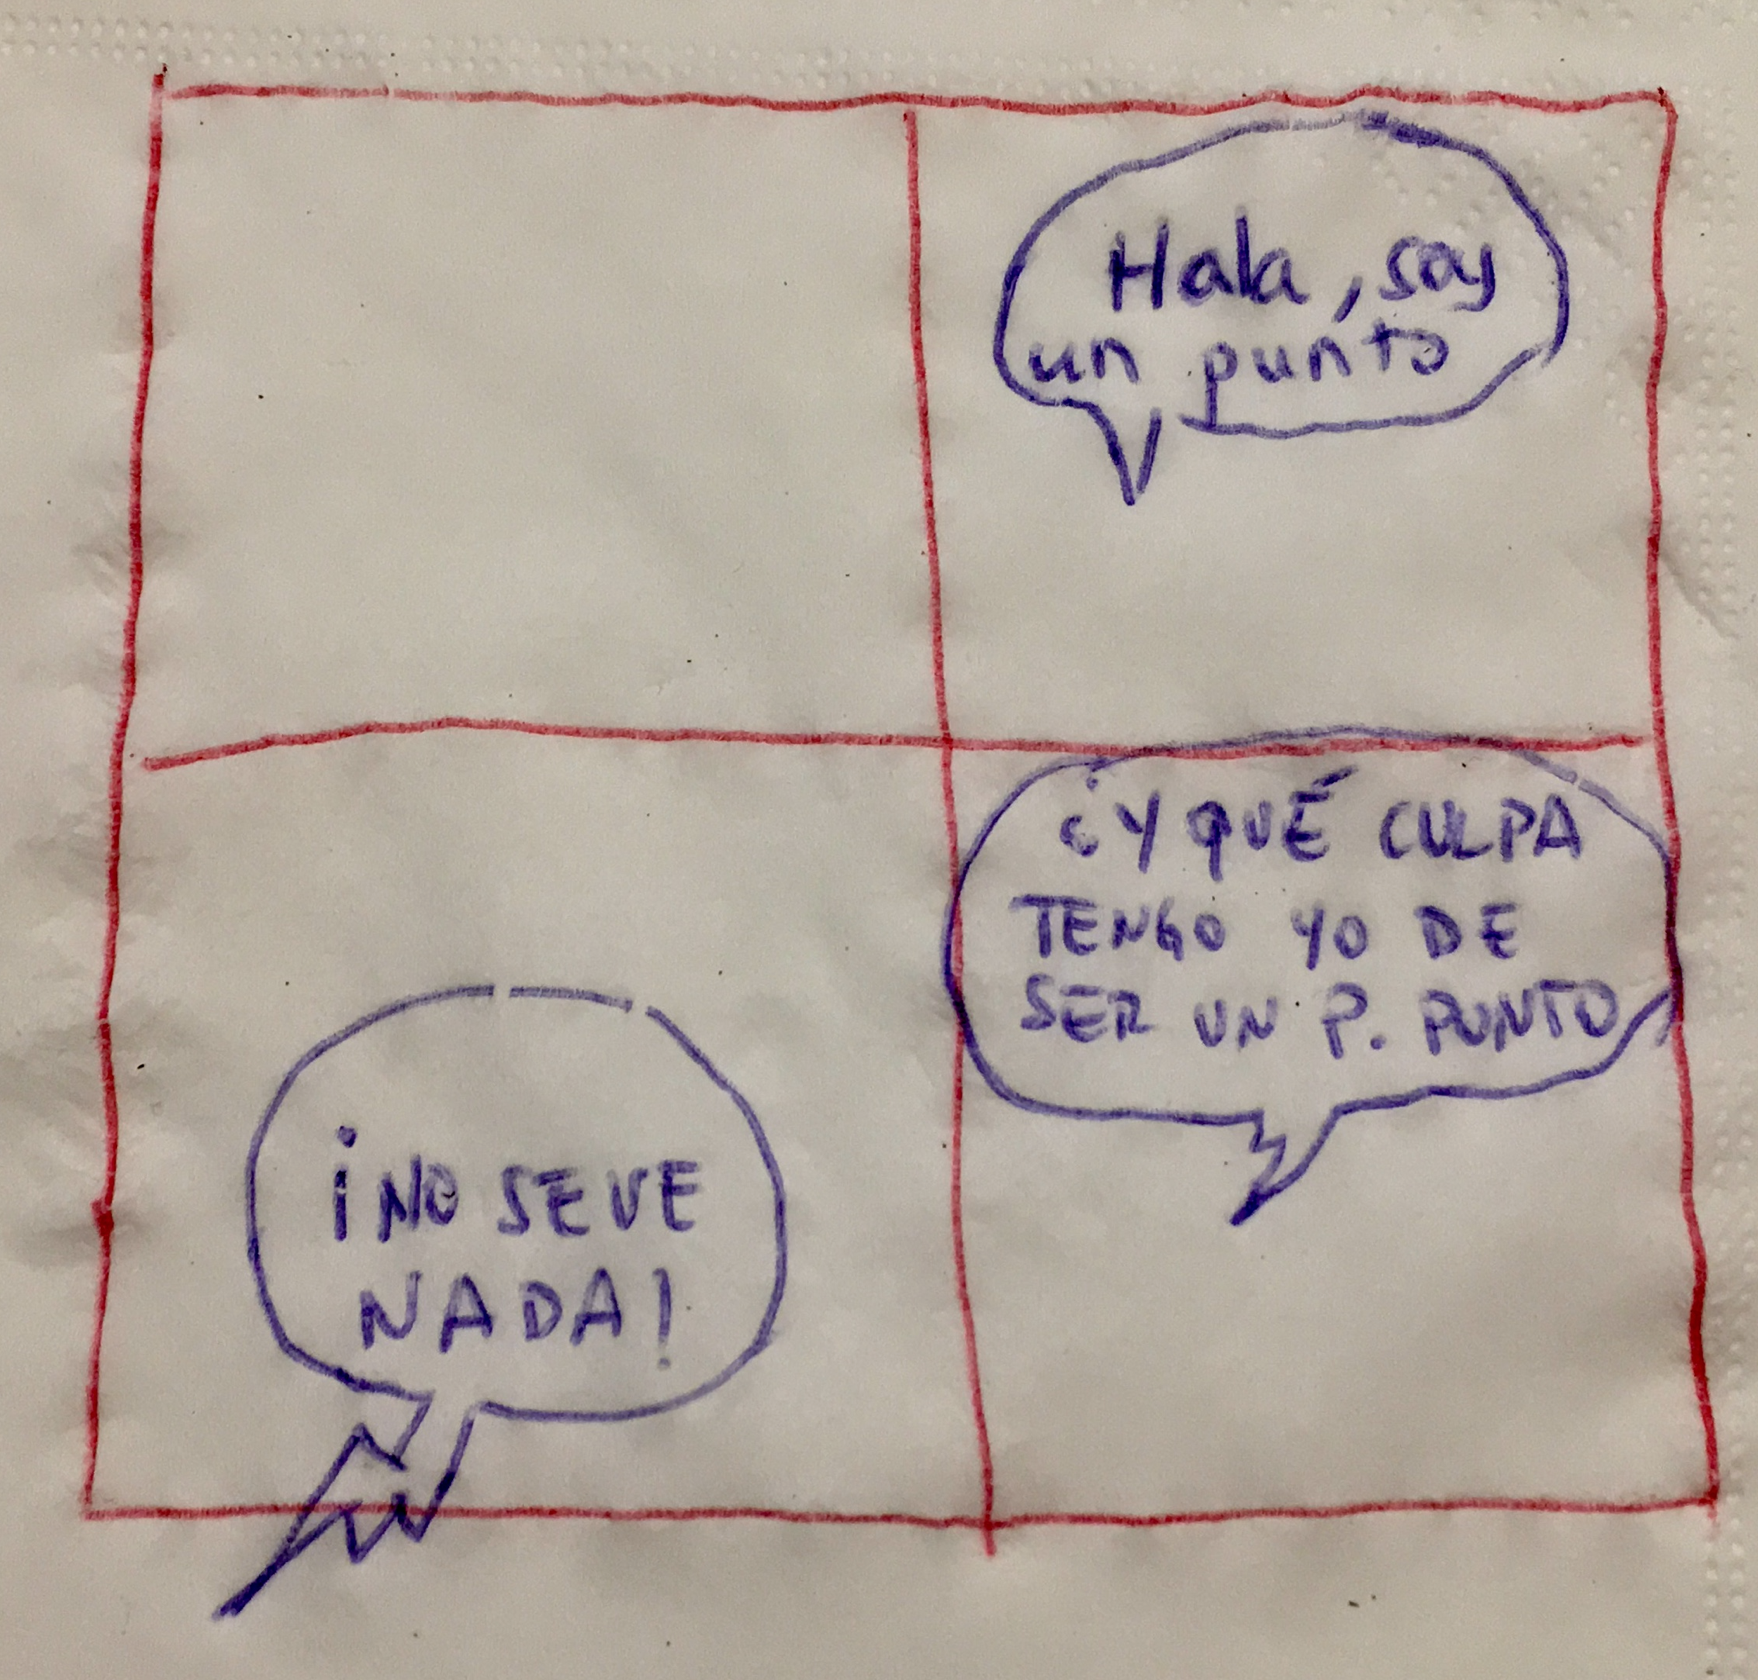
\includegraphics[width=1\textwidth]{imagenes/imagenes11/T11IM39.png}
	\end{figure}

\newpage %***********************************

\section{Resumen}

\begin{myalertblock}{Resumen espació euclideo}

Ángulos:

\begin{itemize}
\item $\theta=\measuredangle(r,s)\equiv \measuredangle(\vec v_r,\vec v_s) \; \to \; \cos \theta = \dfrac {|\;\vec v_r \cdot \vec v_s\;|}{|\vec v_r|\;|\vec v_s|}$

\item $\theta=\measuredangle(\pi,\sigma)\equiv \measuredangle(\vec n_{\pi},\vec n_{\sigma}) \; \to \; \cos \theta = \dfrac {|\;\vec n_{\pi} \cdot \vec n_{\sigma}\;|}{|\vec n_{\pi}|\;|\vec n_{\sigma}|}$

\item $\varphi=\measuredangle(r,\pi)\equiv 90^o-\theta,\;\theta=\measuredangle(\vec v_r,\vec n_{\pi}) \; \to \;$

$\to  \cos \theta = \dfrac {|\;\vec v_r \cdot \vec n_{\pi}\;|}{|\vec v_r|\;|\vec n_{\pi}|}$
\end{itemize}
\line(1,0){250} 

Distancias:

\begin{itemize}
\item $d(P,Q)=|\overrightarrow{PQ}|$ $\qquad$
\item $d(P,r)=\dfrac {|\vec v_r \times \overrightarrow{PP_r}|}{|\vec v_r|}$

\item $d(P,\pi)=\dfrac {|\;Ax_0+By_0+Cz_0+D\;|}{|\vec n_{\pi}|}$

\item \begin{small}$d(r,\pi:\; r\;||\; \pi)=d(P_r,\pi)$;$\quad$
$d(\pi,\sigma:\;\pi\;||\;\sigma)=d(P_{\pi},\sigma)$\end{small}

\item $d(r,s)=\dfrac{|\ [\vec{v_r},\ \vec{v_{s}},\ \overrightarrow{P_rP_s}]\ |}{|\ \vec{v_r} \times \vec{v_s} \ |}$
\end{itemize}
\line(1,0){250} 

Proyecciones ortogonales y simétricos.

Recta perpendicular común y plano equidistante de dos rectas que se cruzan.

\end{myalertblock}




%  \hspace{-10mm}\rotatebox{180}{\leftline{\textcolor{gris}{\footnotesize{ $Resp. 1$  }}}\normalsize{.}}